%%%%%%%%%%%%%%%%%%%%%%%%%%%%%%%%%%%%%%%%%
% kaobook
% LaTeX Template
% Version 1.2 (4/1/2020)
%
% This template originates from:
% https://www.LaTeXTemplates.com
%
% For the latest template development version and to make contributions:
% https://github.com/fmarotta/kaobook
%
% Authors:
% Federico Marotta (federicomarotta@mail.com)
% Based on the doctoral thesis of Ken Arroyo Ohori (https://3d.bk.tudelft.nl/ken/en)
% and on the Tufte-LaTeX class.
% Modified for LaTeX Templates by Vel (vel@latextemplates.com)
%
% License:
% CC0 1.0 Universal (see included MANIFEST.md file)
%
%%%%%%%%%%%%%%%%%%%%%%%%%%%%%%%%%%%%%%%%%

%----------------------------------------------------------------------------------------
%	PACKAGES AND OTHER DOCUMENT CONFIGURATIONS
%----------------------------------------------------------------------------------------

\documentclass[
	fontsize=10pt, % Base font size
	twoside=false, % Use different layouts for even and odd pages (in particular, if twoside=true, the margin column will be always on the outside)
	%open=any, % If twoside=true, uncomment this to force new chapters to start on any page, not only on right (odd) pages
	%chapterprefix=true, % Uncomment to use the word "Chapter" before chapter numbers everywhere they appear
	%chapterentrydots=true, % Uncomment to output dots from the chapter name to the page number in the table of contents
	numbers=noenddot, % Comment to output dots after chapter numbers; the most common values for this option are: enddot, noenddot and auto (see the KOMAScript documentation for an in-depth explanation)
	%draft=true, % If uncommented, rulers will be added in the header and footer
	%overfullrule=true, % If uncommented, overly long lines will be marked by a black box; useful for correcting spacing problems
	UTF8,
	]{kaobook}

% Choose the language
\usepackage[UTF8]{ctex}
\usepackage[english]{babel} % Load characters and hyphenation
\usepackage[english=british]{csquotes}	% English quotes

\usepackage{indentfirst}%首段空格

\usepackage{xeCJK}
\setCJKmainfont {FangSong}
\setCJKsansfont {FangSong}
\setCJKmonofont {FangSong}
% Load packages for testing
\usepackage{blindtext}
%\usepackage{showframe} % Uncomment to show boxes around the text area, margin, header and footer
%\usepackage{showlabels} % Uncomment to output the content of \label commands to the document where they are used

% Load the bibliography package
\usepackage{styles/kaobiblio}
\addbibresource{main.bib} % Bibliography file

% Load mathematical packages for theorems and related environments. NOTE: choose only one between 'mdftheorems' and 'plaintheorems'.
\usepackage{styles/mdftheorems}
%\usepackage{styles/plaintheorems}

\graphicspath{{examples/documentation/images/}{images/}} % Paths in which to look for images

\makeindex[columns=3, title=Alphabetical Index, intoc] % Make LaTeX produce the files required to compile the index

\makeglossaries % Make LaTeX produce the files required to compile the glossary

\makenomenclature % Make LaTeX produce the files required to compile the nomenclature

% Reset sidenote counter at chapters
%\counterwithin*{sidenote}{chapter}

%----------------------------------------------------------------------------------------

\begin{document}

%----------------------------------------------------------------------------------------
%	BOOK INFORMATION
%----------------------------------------------------------------------------------------


\title{关于物联网智能家居的研究与实践}
\subtitle{物联网智能开关电路的设计与实现}

\author{周子钰}

\date{二〇二〇年八月一日}

\publishers{山东省青岛第十七中学}

%----------------------------------------------------------------------------------------

\frontmatter % Denotes the start of the pre-document content, uses roman numerals

%----------------------------------------------------------------------------------------
%	OPENING PAGE
%----------------------------------------------------------------------------------------

%\makeatletter
%\extratitle{
%	% In the title page, the title is vspaced by 9.5\baselineskip
%	\vspace*{9\baselineskip}
%	\vspace*{\parskip}
%	\begin{center}
%		% In the title page, \huge is set after the komafont for title
%		\usekomafont{title}\huge\@title
%	\end{center}
%}
%\makeatother

%----------------------------------------------------------------------------------------
%	COPYRIGHT PAGE
%----------------------------------------------------------------------------------------

\makeatletter

\lowertitleback{
	\textbf{版权声明}\\
	本研究课题、研究成果、研究报告之版权归属于原作者:周子钰(山东省青岛第十七中学,2019级十班)。未经原作者允许,不得复制、转载本文内容,否则将视为侵权;如需引用本文内容,请写明来源及其原作者。对于不遵守此声明或者其它违法使用本文内容者,本人依法保留追究权等。
	
	\medskip
	
	\textbf{鸣谢}\\
	本报告使用 \href{https://sourceforge.net/projects/koma-script/}{\KOMAScript}与\href{https://www.latex-project.org/}{\LaTeX}编写与排版;模板套用\href{https://github.com/fmarotta/kaobook/}{kaobook},以上开放源代码;本报告所用模板之源代码可见于:\\\url{https://github.com/fmarotta/kaobook}。
	
	\medskip
	
	本课题研究成果之代码与原理图等均遵照GNU General Public License v3.0开源于Github:\url{https://github.com/JunASAKA/IoT-Relay_Researching/},其版权所有于周子钰(@JunASAKA);请自觉遵守开源协议,对于不遵守开源协议者,本人依法保留追究权等。
}
\makeatother

%----------------------------------------------------------------------------------------
%	DEDICATION
%----------------------------------------------------------------------------------------

\dedication{
	Given enough eyeballs, all bugs are shallow.\\
	\flushright ——Linus Torvalds
}

%----------------------------------------------------------------------------------------
%	OUTPUT TITLE PAGE AND PREVIOUS
%----------------------------------------------------------------------------------------

% Note that \maketitle outputs the pages before here

% If twoside=false, \uppertitleback and \lowertitleback are not printed
% To overcome this issue, we set twoside=semi just before printing the title pages, and set it back to false just after the title pages
\KOMAoptions{twoside=semi}
\maketitle
\KOMAoptions{twoside=false}

%----------------------------------------------------------------------------------------
%	PREFACE
%----------------------------------------------------------------------------------------

%\input{chapters/preface.tex}

%----------------------------------------------------------------------------------------
%	TABLE OF CONTENTS & LIST OF FIGURES/TABLES
%----------------------------------------------------------------------------------------

\begingroup % Local scope for the following commands

% Define the style for the TOC, LOF, and LOT
%\setstretch{1} % Uncomment to modify line spacing in the ToC
%\hypersetup{linkcolor=blue} % Uncomment to set the colour of links in the ToC
\setlength{\textheight}{23cm} % Manually adjust the height of the ToC pages

% Turn on compatibility mode for the etoc package
\etocstandarddisplaystyle % "toc display" as if etoc was not loaded
\etocstandardlines % toc lines as if etoc was not loaded

\tableofcontents % Output the table of contents

\listoffigures % Output the list of figures

% Comment both of the following lines to have the LOF and the LOT on different pages
\let\cleardoublepage\bigskip
\let\clearpage\bigskip

%\listoftables % Output the list of tables

\endgroup

%----------------------------------------------------------------------------------------
%	MAIN BODY
%----------------------------------------------------------------------------------------

\mainmatter % Denotes the start of the main document content, resets page numbering and uses arabic numbers
\setchapterstyle{kao} % Choose the default chapter heading style

\setchapterpreamble[u]{\margintoc}
\chapter{介绍}
\labch{intro}

声明:本课题的研究秉承开源的理念,除Apple HomeKit相关项目(商用软件)外,本课题所选择的操作系统、应用程式均为开放源码软件系统。另,本课题中设计的硬件电路等设备也均开源。

\section{研究背景}
\setlength\parindent{2em} 信息技术的不断发展,催生出一个新的概念——物联网(Internet of Things, IoT)\sidenote[][90mm]{The Internet of things (IoT) is a system of interrelated computing devices, mechanical and digital machines provided with unique identifiers (UIDs) and the ability to transfer data over a network without requiring human-to-human or human-to-computer interaction.}。即将生活中原本须手动操作的物品接入网路,以实现自动化、智能化、集中化的管理与操控。在这种情况下,各大互联网厂商都对此提出过或多或少的物联网解决方案。可以说,它已经深入到了人们的生活中。
\par 众多物联网产品中——大概是由于产品定位或专利等影响吧——普遍地价格很高,哪怕是一个简单的遥控灯泡,也要数十元钱;想把它们带到日常生活中去使用,可不是一件简单的事情——至少我是这么认为的。
\par 于是,如何用更低的成本达到相同甚至更好的效果,就是我要去思考与研究的了,问题由此产生。

\section{研究大致流程}
\par 众多物联网设备中,应用最广泛的应该是智能开关、智能灯泡等基础生活用电器;对于这些设备甚至更复杂的设备,其核心在于通过网络控制其工作状态。换句话说,大部分设备中不可缺少的部分,就是一个由网络控制的开关电路。这,也就是我们要设计的对象。
\par 本课题将从思路的提出开始,对硬件、电路的选材、设计、部署等;对软件及应用程式的适配、编译、烧录等步骤进行操作与记录;以达到在实践中研究、在研究中学习的目的。

\section{研究目的} 
\begin{itemize}
	\item 了解物联网最新发展情况
	\item 利用电学与信息技术学等知识,设计、制造、部署自己的物联网设备
	\item 开拓思路,寻找与设计更优秀的解决方案
	\item ……
\end{itemize}

\section{有关技术}
\begin{itemize}
	\item 基础PCB印刷线路板的设计
	\item 微型控制单元(单片机)、微型计算机等相关知识
	\item 底层程式设计
	\item 无线网络有关软硬件知识
	\item ……
\end{itemize}

\begin{marginfigure}[1.5cm]
	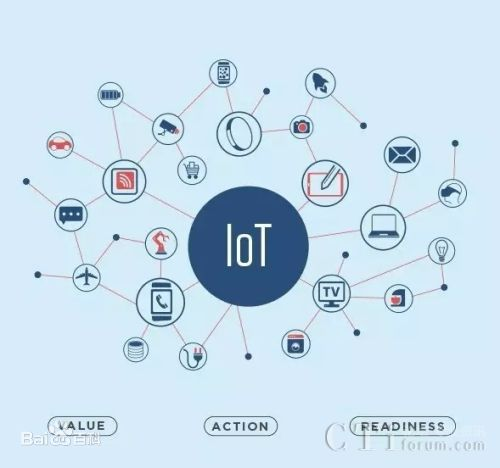
\includegraphics{iot}
	\caption[iot]{The IoT.\\ 
	\url{https://bkimg.cdn.bcebos.com/pic/562c11dfa9ec8a13e355fe69f903918fa1ecc0e8?x-bce-process=image/watermark,image_d2F0ZXIvYmFpa2U4MA==,g_7,xp_5,yp_5}}
\end{marginfigure}



\pagelayout{wide} % No margins
\addpart{设计思路与解决方案}
\pagelayout{margin} % Restore margins

\setchapterpreamble[u]{\margintoc}
\chapter{硬件层面的解决方案}
\labch{hardware}

\setlength\parindent{2em} 本章将介绍本课题中硬件的设计思路、硬件主体与其它元器件的选材、电路规划与PCB印刷线路板的设计。包括电路实现方式、连接方式、工作流程以及对电路所做的兼容性、安全性、易修复性的优化。

\section{设计思路}

\setlength\parindent{2em} 本次研究最终要达到的目的是通过网络控制电路的通断,所以大概的方向就是将带有无线网络接收(或发射)功能的微控制单元(Microcontroller Unit, MCU;或称为单片机)\sidenote{微控制单元,是把中央处理器的频率与规格做适当缩减,并将内存、计数器、UART等周边接口,整合在单一芯片上,形成芯片级的计算机,为不同的应用场合做不同组合控制。\\以下称为单片机},或者是可以通过其他电路实现此功能的单片机进行编程,从而实现对电路的控制。
\par 具体来说,一般的小型单片机都有通用型之输入输出接口(GPIO),可用于控制电路。GPIO既可用于输入,亦可用于输出,但对与此研究项目来说,只会用到它的输出功能,即调整某些引脚电位的高低来对外部电路造成影响从而实现输出的目的。本研究项目所用的实现方法是通过改变GPIO的电位来造成外电路中部分电路的电位差从而使电流流过光电耦合器\sidenote{光电耦合器是以光为媒介传输电信号的一种电一光一电转换器件。它由发光源和受光器两部分组成。把发光源和受光器组装在同一密闭的壳体内,彼此间用透明绝缘体隔离。发光源的引脚为输入端,受光器的引脚为输出端,常见的发光源为发光二极管,受光器为光敏二极管、光敏三极管等等。}以控制另一部分电路的通断。将这一部分电路作为继电器的输入回路;在此之前,可以用一个金氧半场效晶体管来对电流方向进行管理和限制。
\par 大概的设计思路如此。除这种用单片机与无线网络实现之外,还可以用蓝牙、传感器、磁敏、光敏电阻等配合逻辑电路实现。但考虑到成本、技术要求,特别是便携程度与兼容性,最后选择了单片机用于此课题的研究与实践。

\section{选材与电路概念规划}

\setlength\parindent{2em} 由于本研究项目中对单片机的功能要求较为单一,所以选择了ESP8266-01S(以下简称为ESP01S)作为微控单元,其本身也可以作为无线网络模块连接与51单片机等通信。ESP01S的工作电压为3.3V。至于继电器,就选择常用的SRD-05VC-SL-C,其共有五个引脚,其中两个是线圈的引脚,另外三个分别是常闭端(NC)、常开端(NO)和公共端(COM)。其驱动电压为5V,最大允许10A,250V交流电通过,所以用来控制交流220V市电很合适。
\par 至此,所要设计的电路的输入与输出端有哪些,基本可以确定。除去天线以外,需要有一个电源输入以给单片机以及继电器电路供电。由于ESP01S的工作电压为3.3V,继电器控制电压为5V;所以总输入电压选择5V或者12V,这两种电压很容易获得,且可以通过降压来保证各个元件正常工作。最终确定为5V总电压,输入后通过LD1117芯片降成3.3V供予MCU(\reffig{normalconcept})。

\begin{figure*}[h!]
	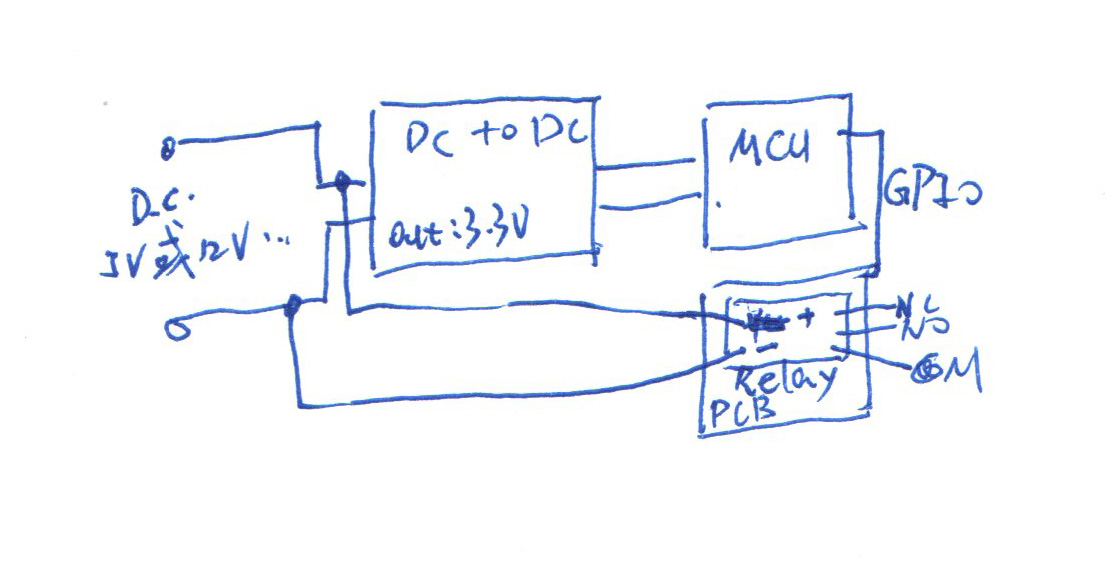
\includegraphics[width=\textwidth]{concept}
	\caption[concept]{电路的概念图}
	\labfig{normalconcept}
\end{figure*}

\begin{marginfigure}[-0.5cm]
	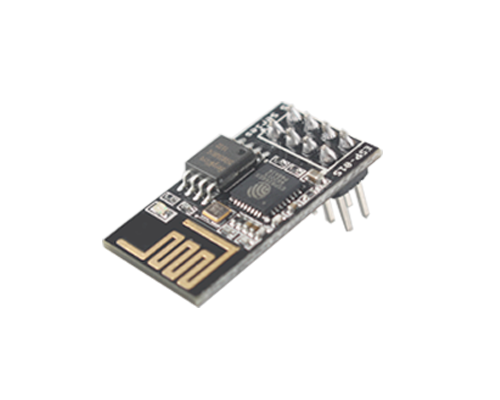
\includegraphics{esp01s}
	\caption[esp01s]{The ESP01S}
\end{marginfigure}

\begin{marginfigure}[0cm]
	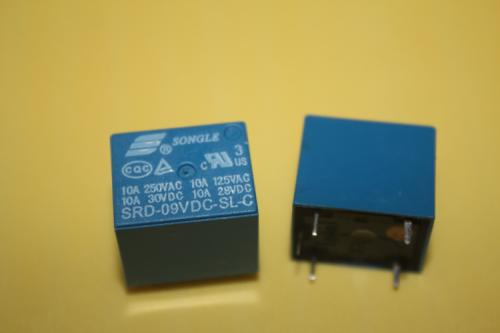
\includegraphics{relay}
	\caption[relay]{The SRD-05VC-SL-C}
\end{marginfigure}

%\begin{kaobox}[frametitle=To Do]
%Implement the \Option{justified} and \Option{margin} options. To be 
%consistent with the \KOMAScript\xspace style, they should accept a 
%simple switch as a parameter, where the simple switch should be 
%\Option{true} or \Option{false}, or one of the other standard values for 
%simple switches supported by \KOMAScript. See the \KOMAScript\xspace 
%documentation for further information.
%\end{kaobox}

\par 电路的大致概念如图\reffig{normalconcept}所示。输入电压为5V(可以通过USB供电),经过降压得到3.3V电压,供予MCU;继电器电路与降压芯片并联,得到5V电压;继电器电路与MCU之间通过GPIO通信。但图中还未给出具体细节,下一步就是对具体的电路进行规划与设计。\\
以下是本研究项目所用到的元器件:

\begin{itemize}
	\item ESP10S
	\item SRD-05VC-SL-C
	\item LD1117
	\item PC817光电耦合器
	\item 2n7002金氧半场效晶体管
	\item (发光)二极管数个
	\item 电容数个
	\item 电阻数个
	\item 电键
\end{itemize}

\section{电路图绘制}

\setlength\parindent{2em} 根据概念图,将LD1117的输入端和继电器线圈的一端与电源正极相连,其间连接一个1微法拉的电容接地用于滤波;出端再接一个100纳法拉的电容接地用于滤波;接地端连接负极。规定电源负极为电位零点,则LD1117输出端电压为3.3V,可直接供予ESP01S的VCC引脚。在ESP01S上,有一个标记为CH\_PD的引脚,这个引脚——从资料上看——是用来控制芯片的状态的,如果它是低电平,芯片处于关机状态;若是高电平,则芯片正常工作。于是将ESP01S的CH\_PD引脚连接至3.3V的供电,之间放置一个10kΩ的上拉电阻。
\par 为实现GPIO的控制目的,将GPIO与一个10kΩ的起保护作用的电阻串联,再使光电耦合器与一个470R电阻串联后与其并联,使得GPIO的电位变化可以对光电耦合器产生影响。光电耦合器的发射极与N沟道MOSFET\sidenote{金氧半场效晶体管(Metal-Oxide-Semiconductor Field-Effect Transistor, MOSFET)是一种可以广泛使用在模拟电路与数字电路的场效晶体管。MOSFET依照其“通道”(工作载流子)的极性不同,可分为“N型”与“P型” 的两种类型,通常又称为NMOSFET与PMOSFET,其他简称上包括NMOS、PMOS等。}的栅极相连,若光电耦合器通路,MOSFET的源极与漏极也导通,继电器线圈的一端就会接地,与另一端产生5V的电位差,线圈通电,继电器工作。从而实现通过GPIO的电位变化来控制继电器通断的目的。最后用一个发光二极管与线圈并联作为指示灯;设置好RESET电建用于MCU的复位,电路的总体设计基本上就完成了。完整的电路(5V的供电未给出)如图\reffig{normalcircuit}所示:

\begin{figure*}[h!]
	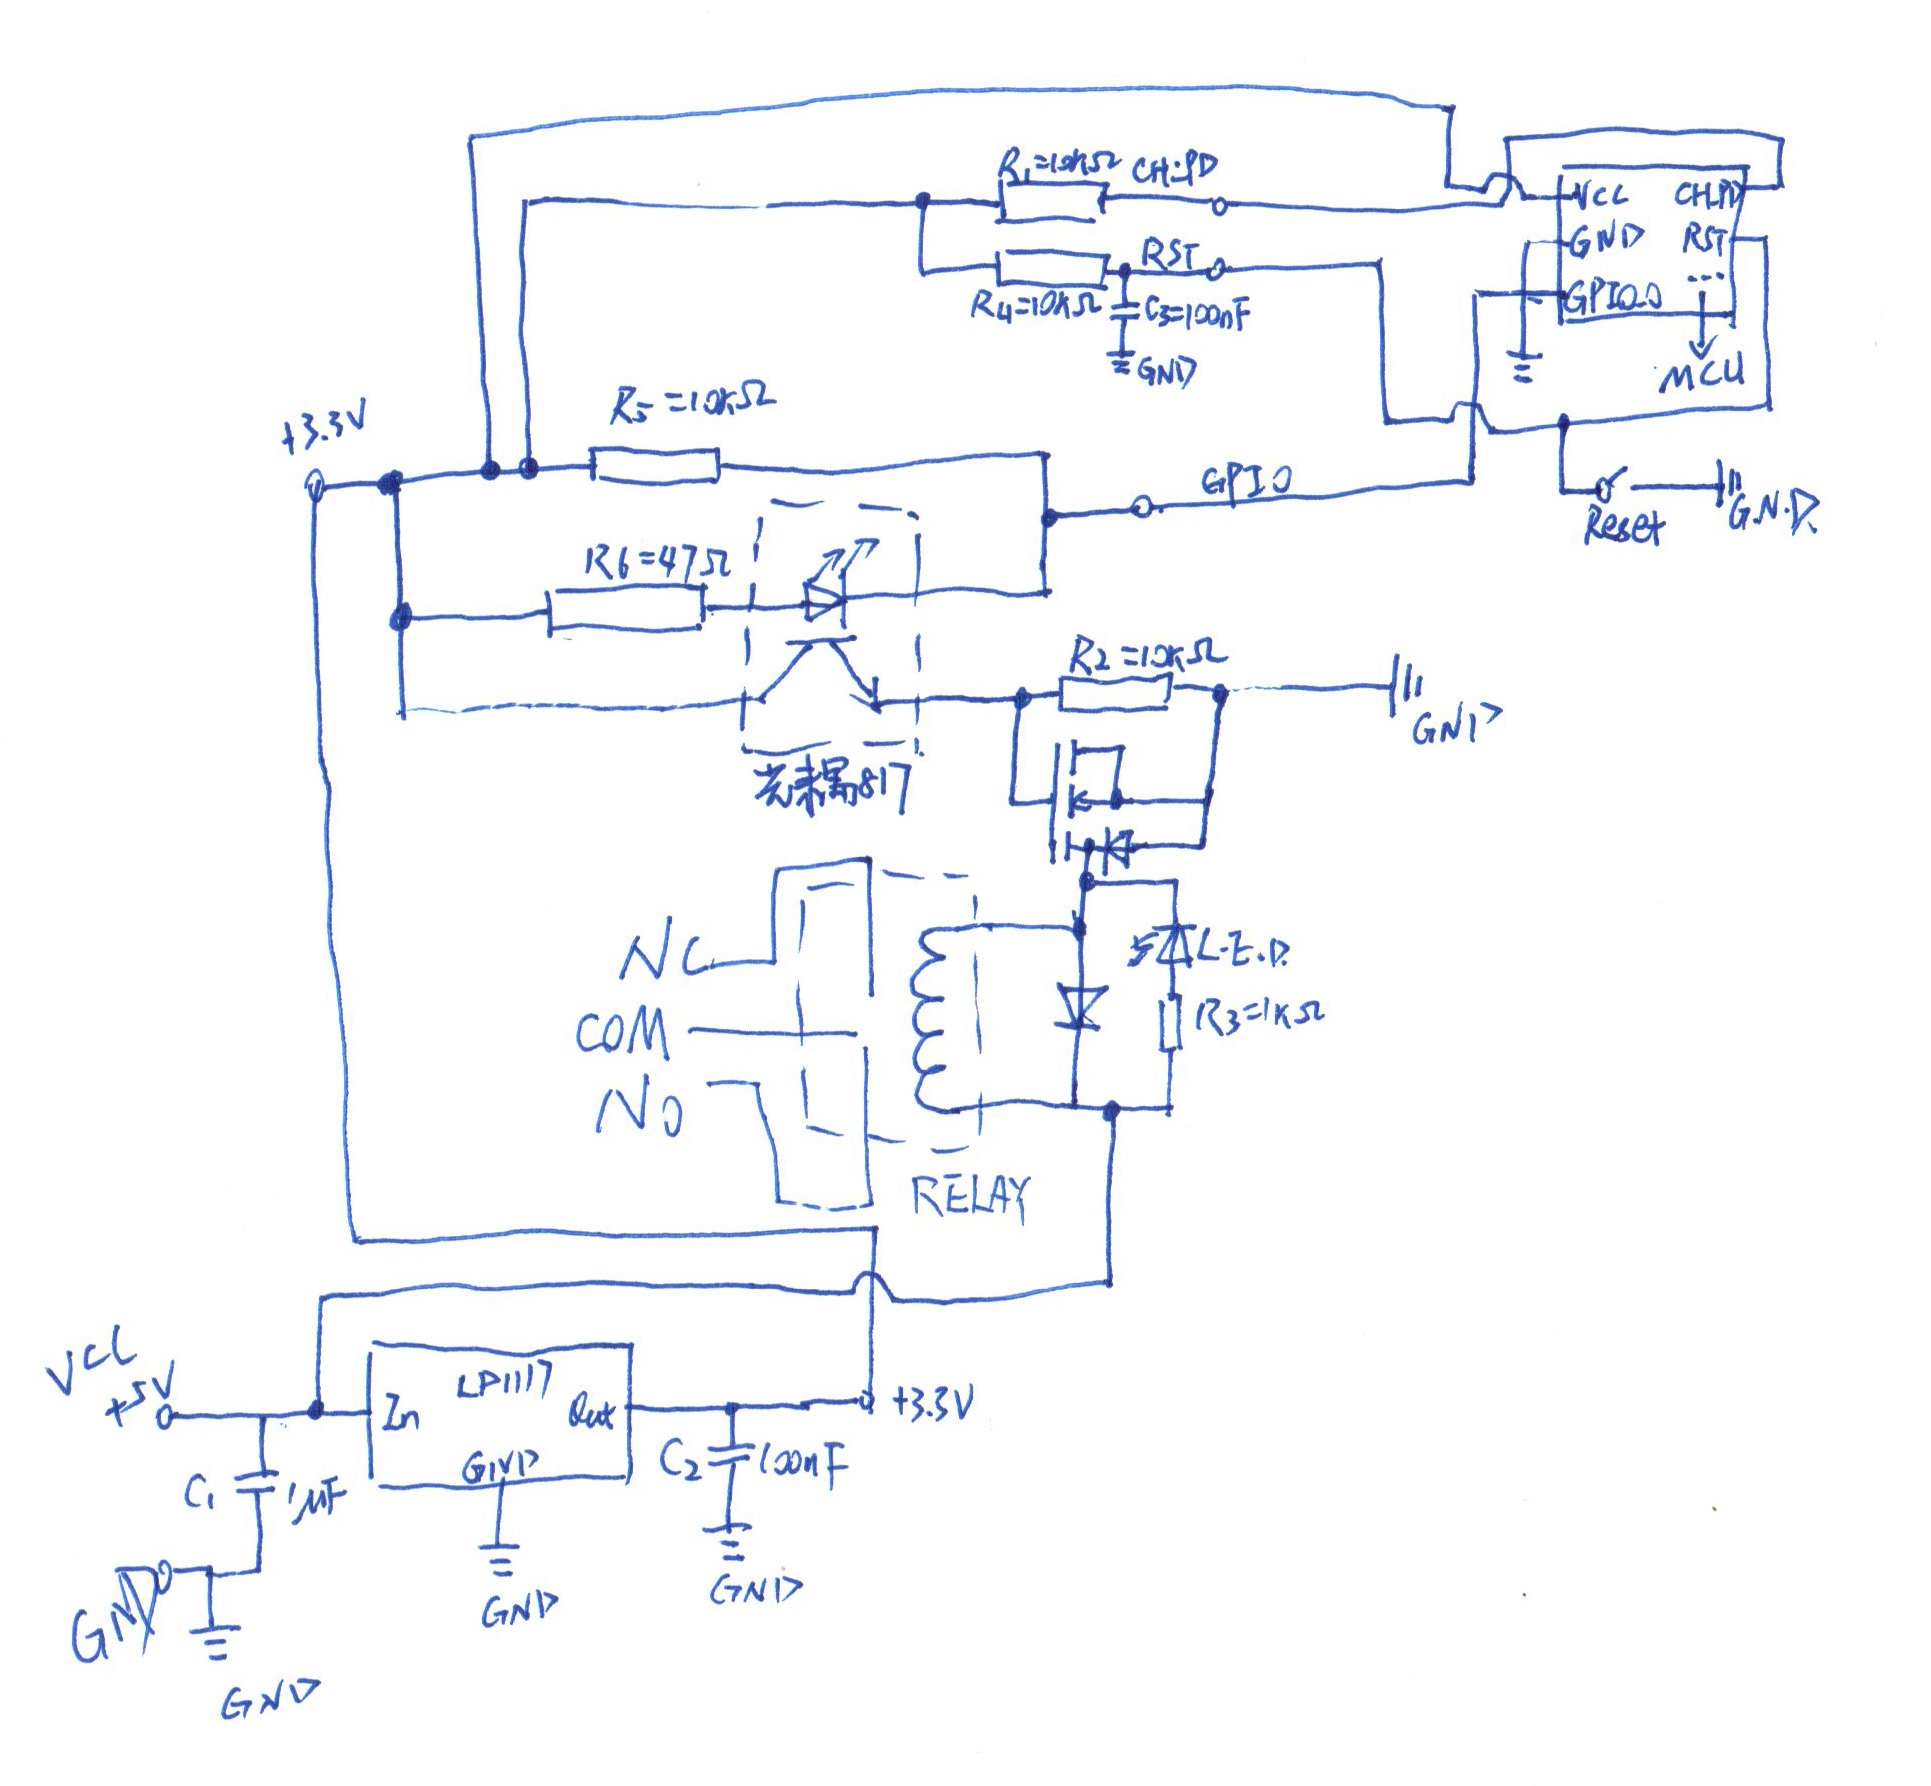
\includegraphics[width=\textwidth]{circuit}
	\caption[circuit]{完整的电路图(5V的供电未给出)}
	\labfig{normalcircuit}
\end{figure*}

\section{依照电路图绘制原理图及设计PCB}

\setlength\parindent{2em} 依照已经绘制完成的电路图,进行PCB印刷线路板的设计。首先需要绘制原理图。上面的电路图大致可以分为四部分:供电部分、单片机部分、光电耦合器部分和继电器部分。依照这个,将电路图中的节点拆分,可以得到原理图。
\par 实际制作时,输入输出接口用端子座实现,所有的接地处,也就是电位为零处,统一接至PCB的地平层。
\par 原理图如图\reffig{normalschematic}所示:
\begin{figure*}[h!]
	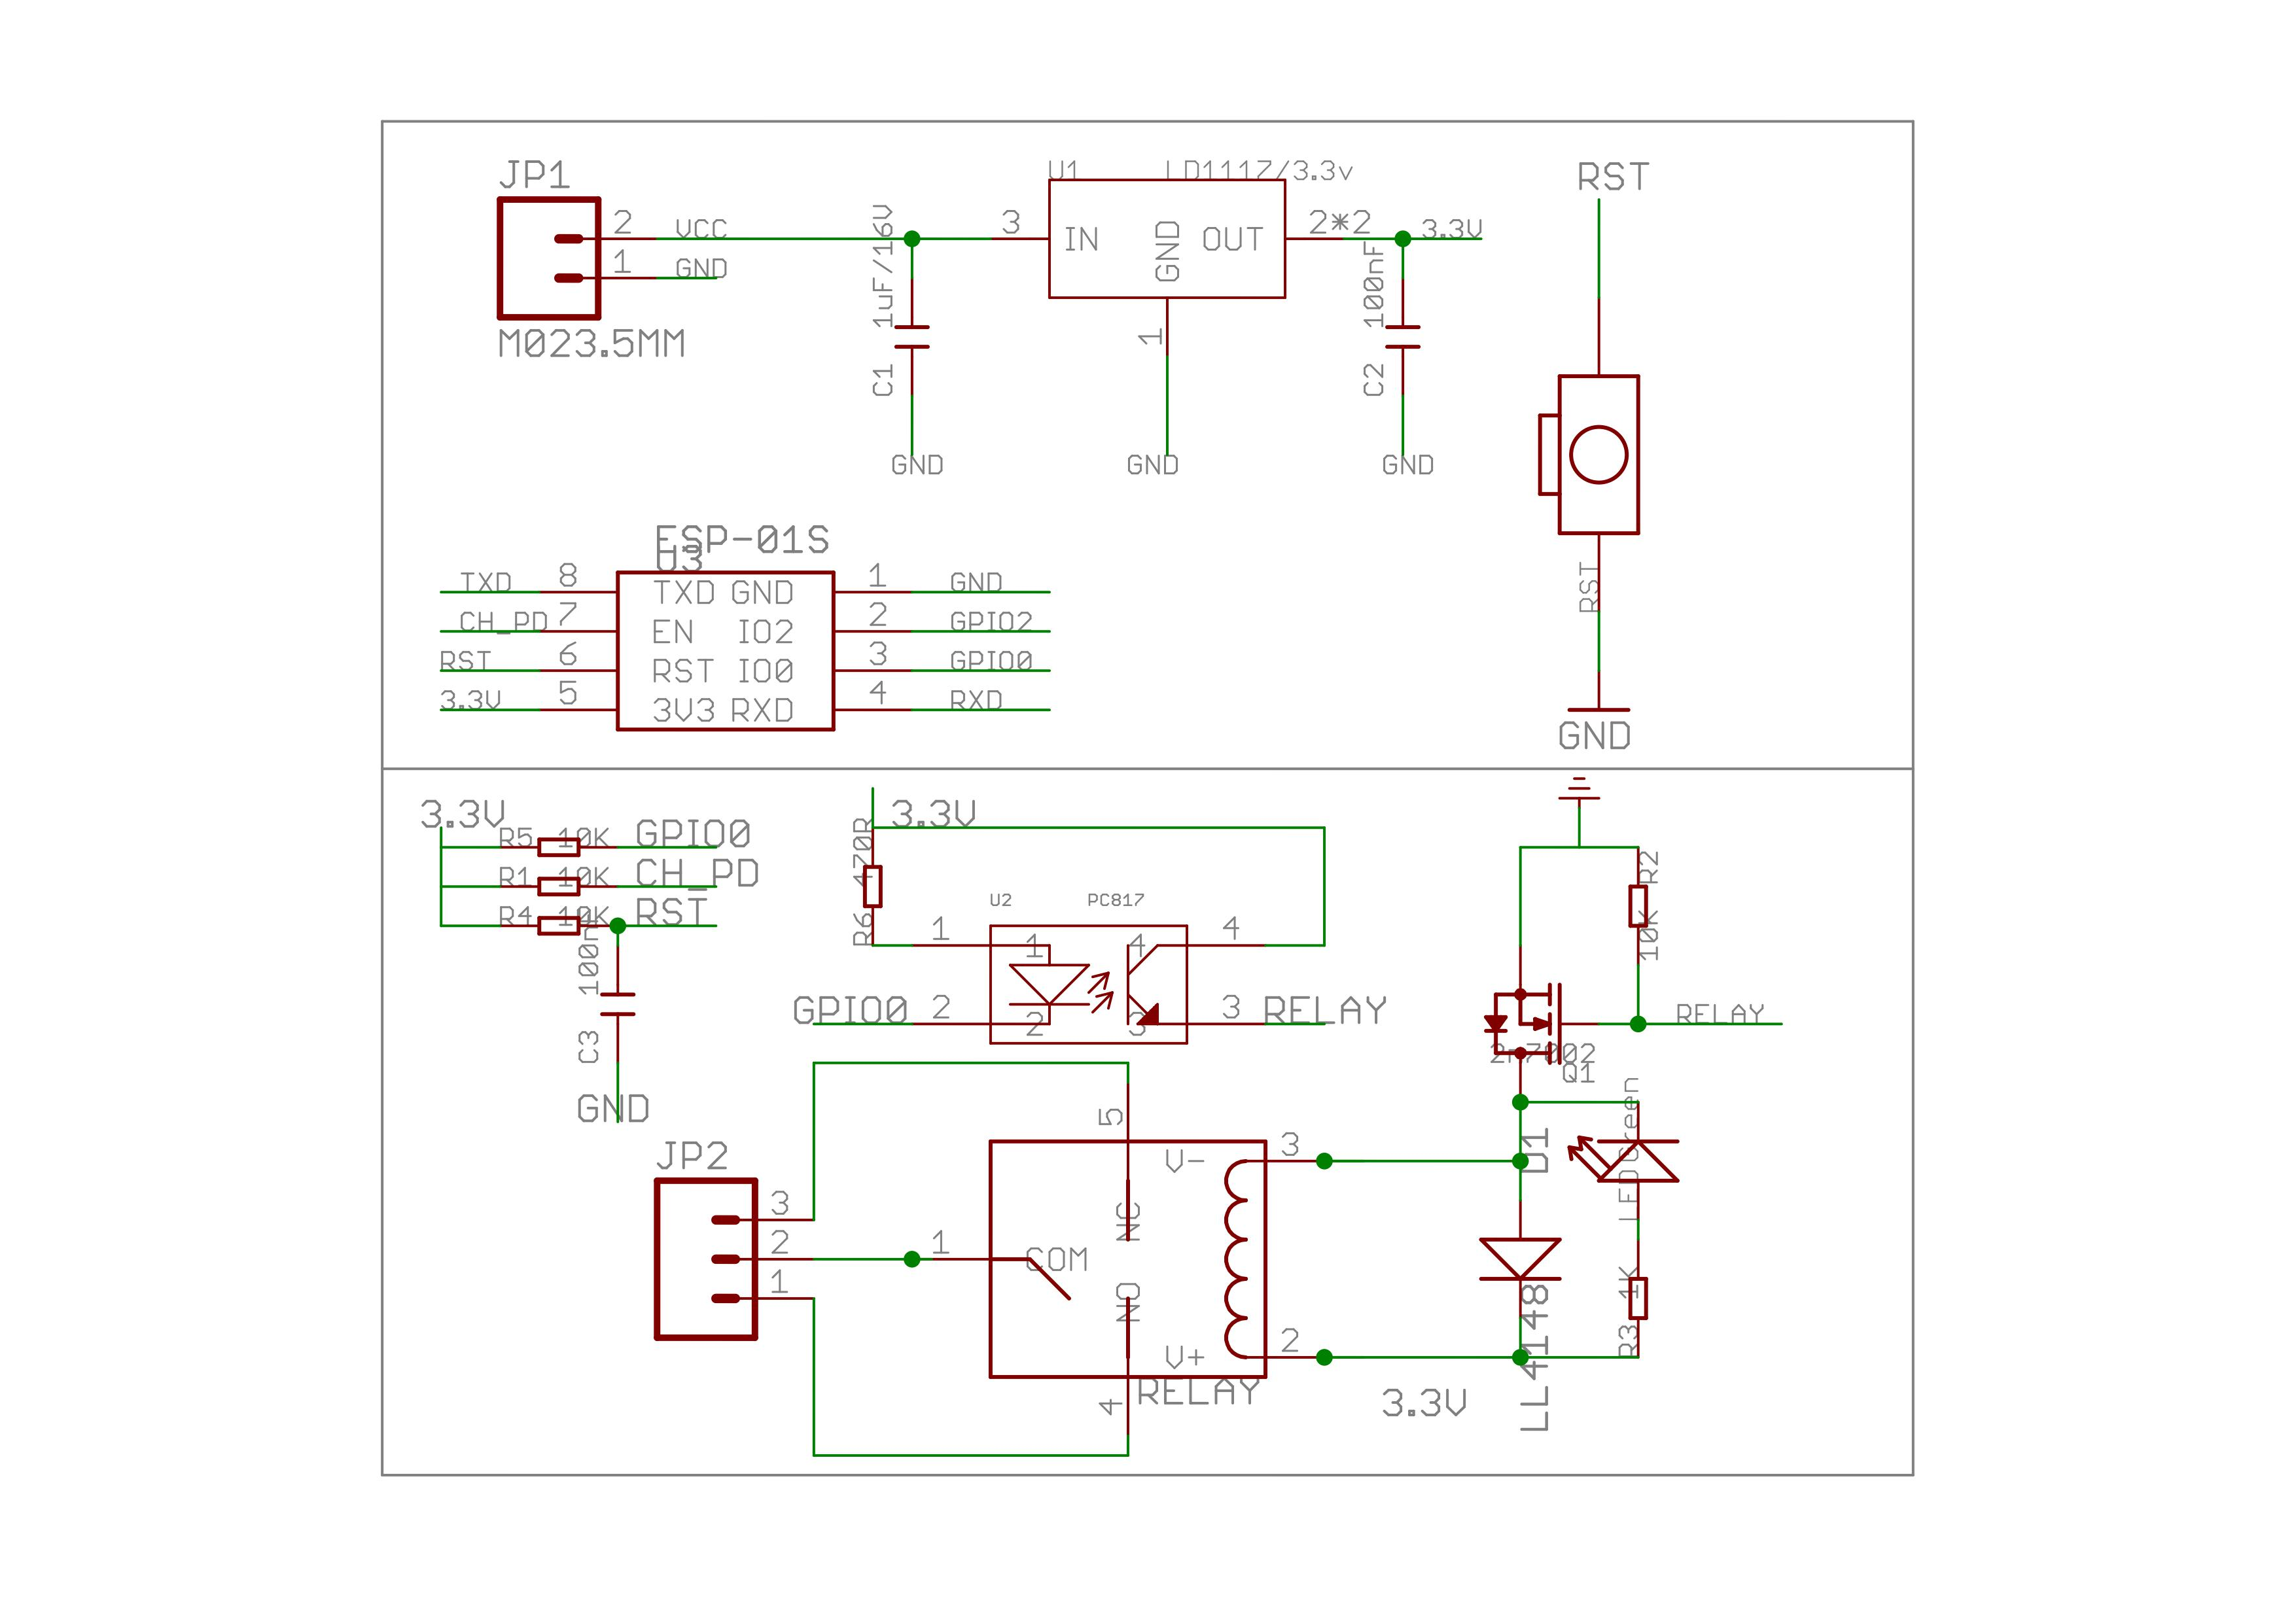
\includegraphics[width=1.5\textwidth]{schematic}
	\caption[schematic]{电路的原理图}
	\labfig{normalschematic}
\end{figure*}
\setchapterpreamble[u]{\margintoc}
\chapter{软件层面的准备}
\labch{software}

\setlength\parindent{2em} 本章将介绍本课题中所用到的软件的选择、编译、配置等过程。包括适配该MCU的操作系统的选择、编译;应用程式的编译、配置;对Apple HomeKik的适配等过程。本课题的研究秉承开源的理念,除Apple HomeKit相关项目(商用软件)外,本课题所选择的操作系统、应用程式均为开放源码软件系统。另,本课题中设计的硬件电路等设备也均开源。

\section{适用于微控单元的实时操作系统}

\setlength\parindent{2em} 既然选择ESP01S当作微控单元,一个合适的操作系统是必要的。考虑到这个项目所要实现的功能,一般的嵌入式操作系统是无法应对的,因为它不具有“实时性”这一大特征。换句话说,从事件的发生到操作系统的响应之间的时间应该受到严格的限制,以保证各个任务能够及时地进行。所以我们需要使用“实时操作系统\sidenote[][-0.5cm]{实时操作系统(RTOS)是指当外界事件或数据产生时,能够接受并以足够快的速度予以处理,其处理的结果又能在规定的时间之内来控制生产过程或对处理系统做出快速响应,调度一切可利用的资源完成实时任务,并控制所有实时任务协调一致运行的操作系统。提供及时响应和高可靠性是其主要特点。}”来适配这个项目。

\par 总的来看,目前有许多操作系统可供选择。比如说$\mu$Clinux、$\mu$C/OS-II、embOS、FreeRTOS等等。其中,$\mu$Clinux的结构相对复杂,而且缺少良好的实时性,故这次未采用。另外,$\mu$C/OS-II、embOS等属于商业操作系统,而非开放源码的系统,灵活度、可移植性大大降低,亦不采用。综上,本研究项目选择了FreeRTOS操作系统。

\begin{marginfigure}[-0.5cm]
	
\includegraphics{freertos}
	\caption[freertos]{Logo of FreeRTOS\\
	\url{https://www.freertos.org/}}
\end{marginfigure}


\par FreeRTOS系统——大概是因为开源——有着诸多的移植版本,几乎适配所有平台,ESP01S也有适配。适用于ESP01S的FreeRTOS之一,也就是本项目所采用的,叫做“ESP-OPEN-RTOS”,来自Github开源平台:\\
\url{https://github.com/SuperHouse/esp-open-rtos}。

\section{ESP-OPEN-RTOS的编译}

\setlength\parindent{2em} 根据ESP-OPEN-RTOS位于Github的官方Wiki中,给出了较为具体的编译步骤,难度不算大,与平常编译Android系统或Linux内核差不多。本次使用的编译平台为Intel x86,操作系统为Kali Linux\sidenote{Kali Linux is an open source project that is maintained and funded by Offensive Security, a provider of world-class information security training and penetration testing services.}。由于Kali Linux中内置较为完整的Linux开发环境,故使用其作为编译主机。编译步骤大致如下:

\begin{marginfigure}[0cm]
	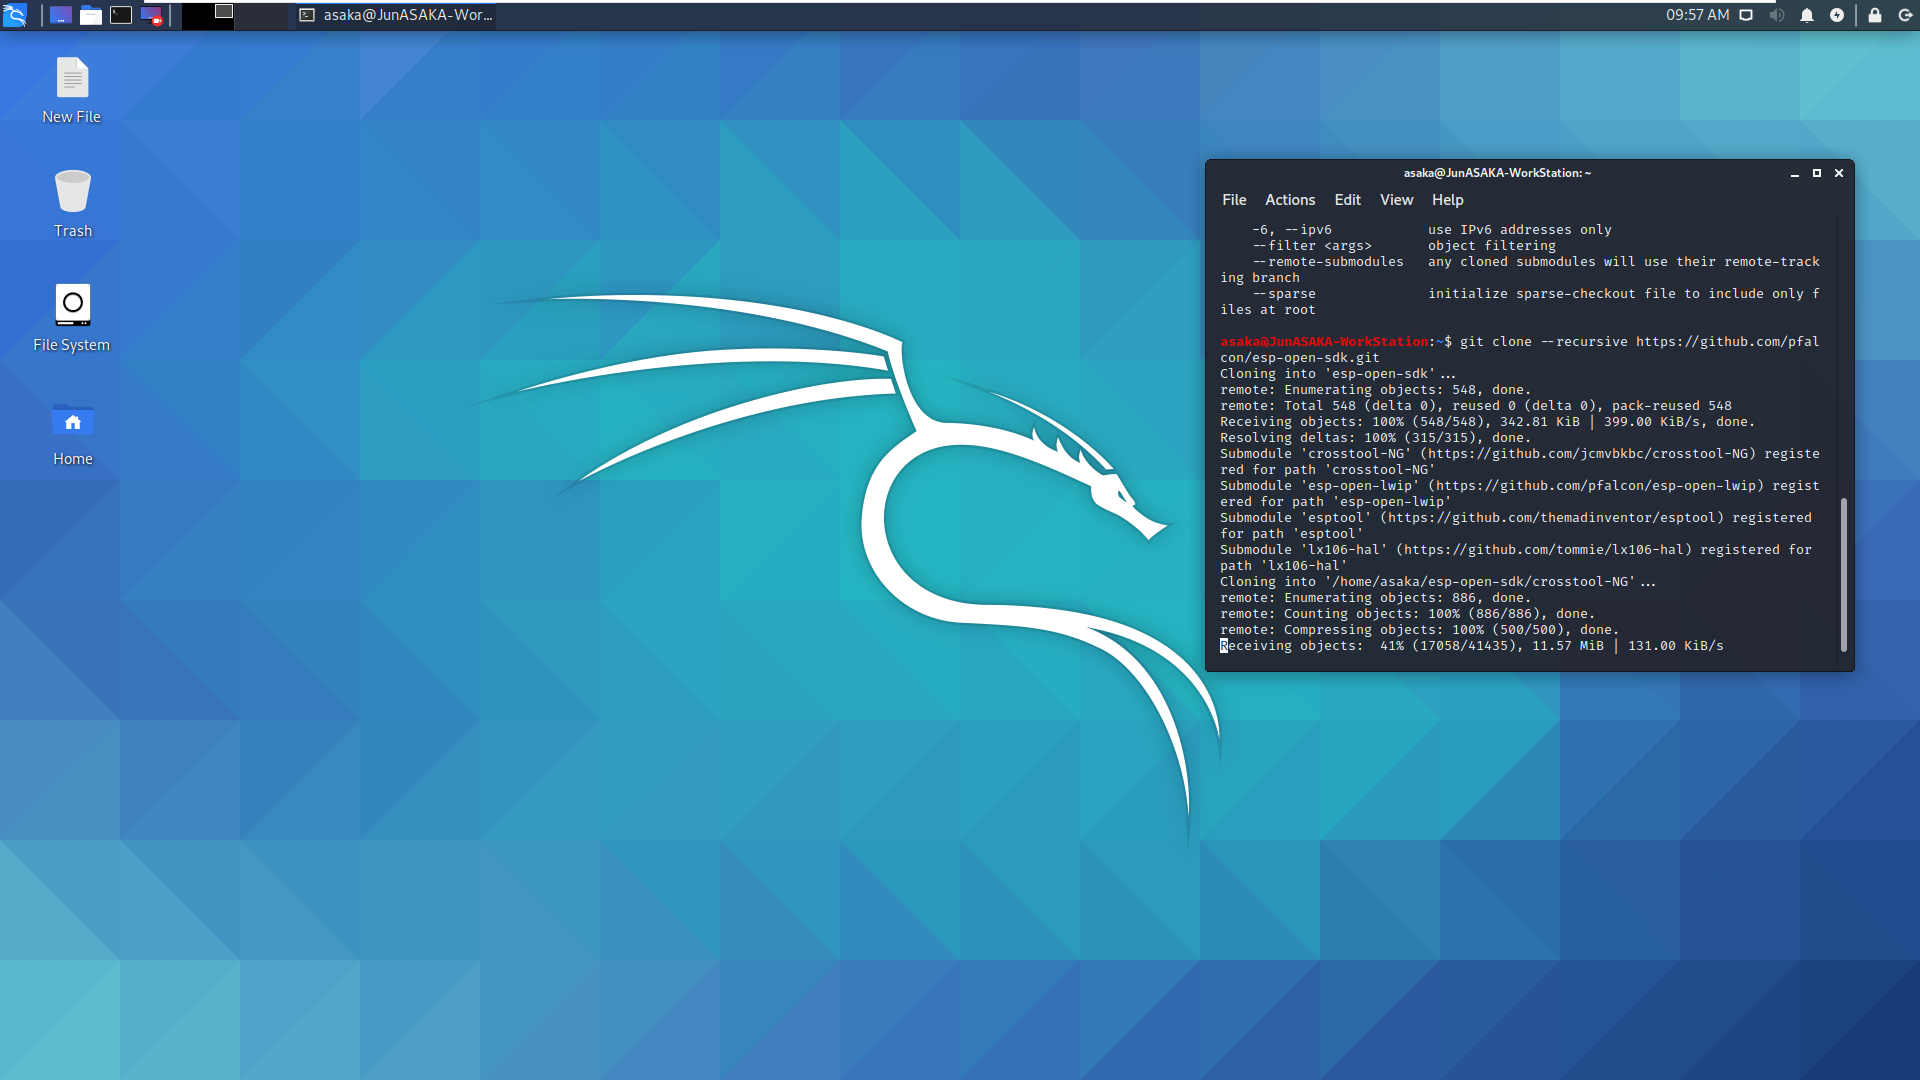
\includegraphics{clone}
	\caption[clone]{RTOS的编译过程}
\end{marginfigure}


\begin{itemize}
	\item 配置适用于ESP的SDK,包括下载SDK源代码并编译适用于主机的二进制文件。
	\item 安装预编译的esptool
	\item 从GitHub克隆源代码
	\item 修改头文件中关于无线网络的配置
	\item 修改其他配置文件
	\item 编译可引导的二进制文件
	\item 烧录(这一步放在后面进行)
\end{itemize}

最后根据Wiki,得到如图\reffig{normalrtosbin}两个二进制文件。

\begin{figure*}[h!]
	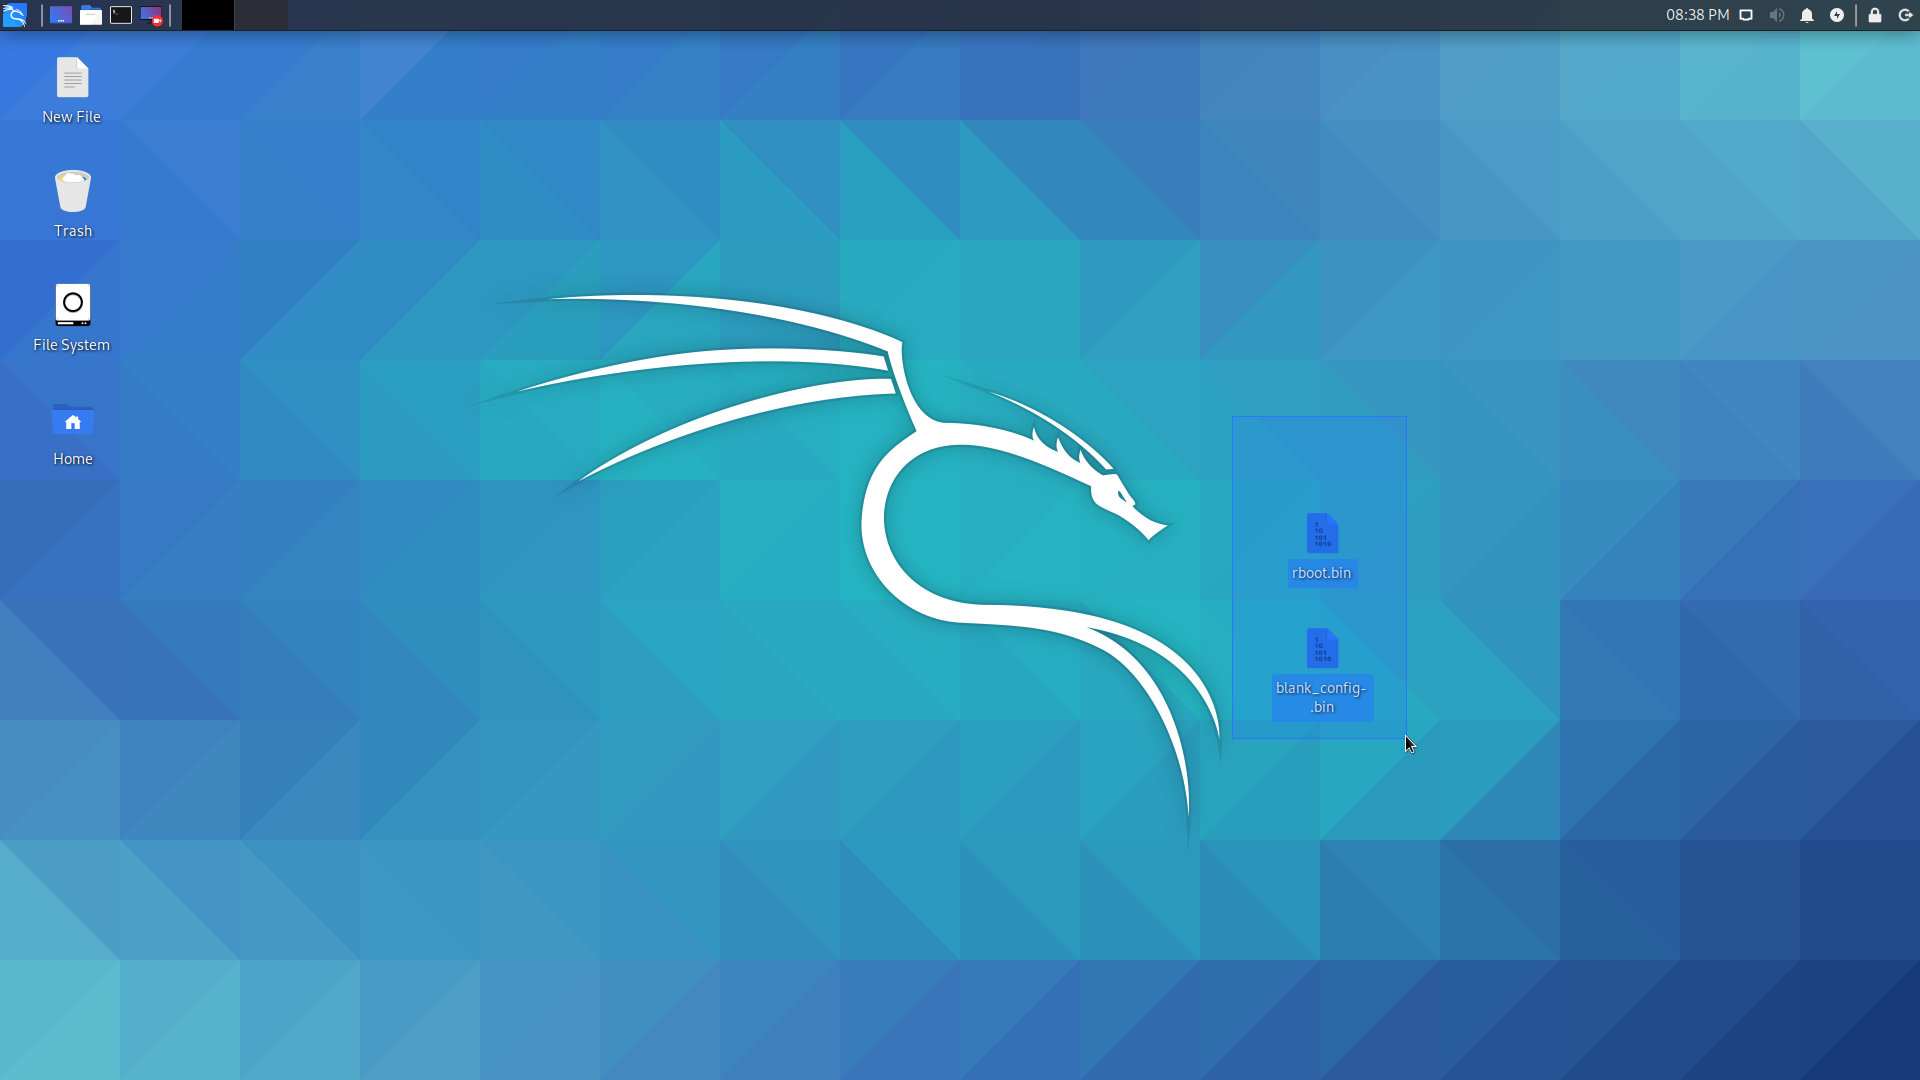
\includegraphics[width=\textwidth]{rtosbin}
	\caption[rtosbin]{编译得到的两个二进制文件}
	\labfig{normalrtosbin}
\end{figure*}

\section{适配于ESP01S以支持Apple HomeKit的应用程式}

\setlength\parindent{2em} 根据Apple Inc.给出的HomeKit Accessory Protocol Specification Non-commercial version\sidenote{\url{https://developer.apple.com/homekit/specification/}},HAP协议是Apple发布的用于Apple智能设备控制物联网智能家居的通讯协议,包含BLE和IP两种方式。为此,本研究项目需要一个适配于ESP01S以让其支持Apple HomeKit通讯协议的应用程式。

\par 在Github上可以找到许多支持HAP的应用程式;其中,本次选择了Home Accessory Architect(以下简称HAA):\url{https://github.com/RavenSystem/esp-homekit-devices}。这次的编译相对来说更简单,仍然需要用到ESP-OPEN-SDK,就像编译RTOS一样;主机操作系统仍是Kali Linux。编译步骤大致如下:

\begin{marginfigure}[0cm]
	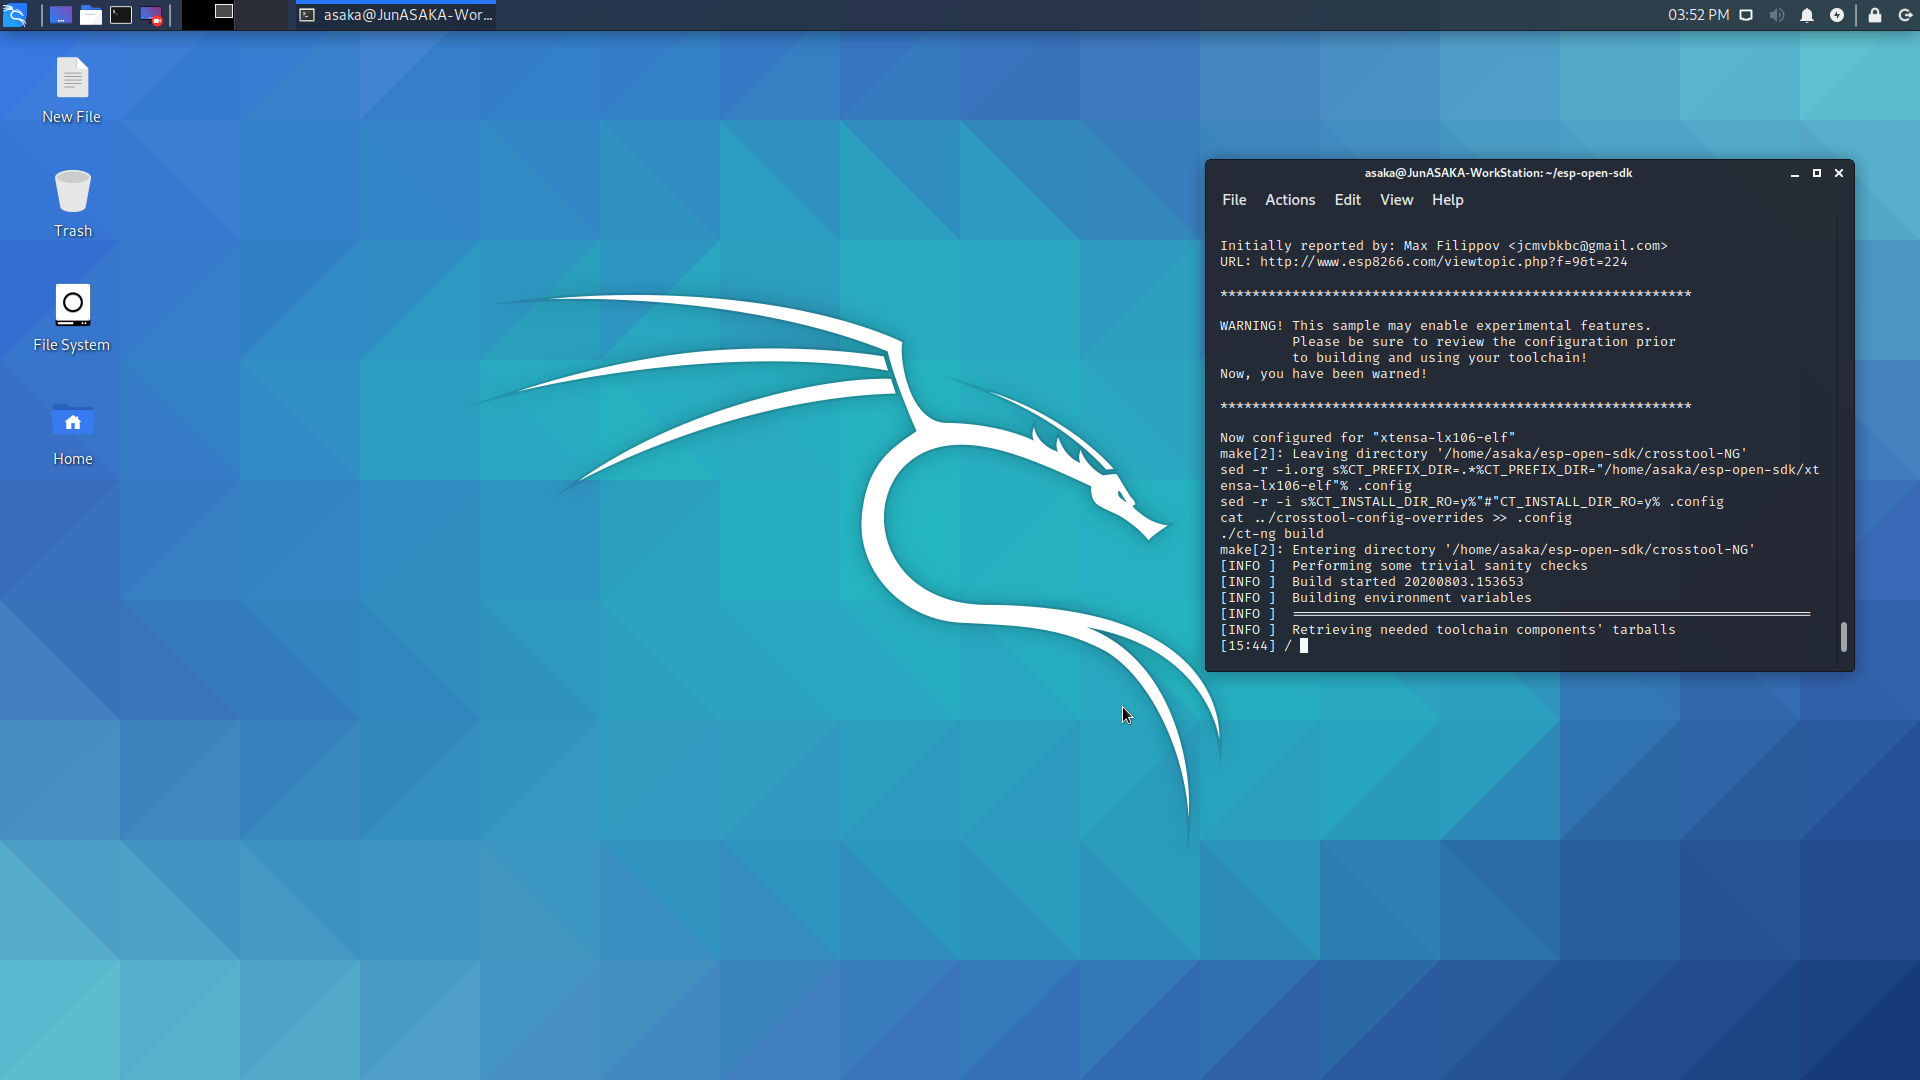
\includegraphics{build}
	\caption[build]{RTOS的编译过程}
\end{marginfigure}

\begin{itemize}
	\item 配置适用于ESP的SDK,上次编译时已经完成了。
	\item 从GitHub克隆源代码
	\item 编译可引导的二进制文件
	\item 安装与配置(这一步放在后面进行)
\end{itemize}

最后得到一个二进制文件。至此,总共编译完成了三个二进制文件如图\reffig{normalbin},包括操作系统和应用程式。接下来将介绍将它们烧录到微控单元并配置的过程。

\begin{figure*}[h!]
	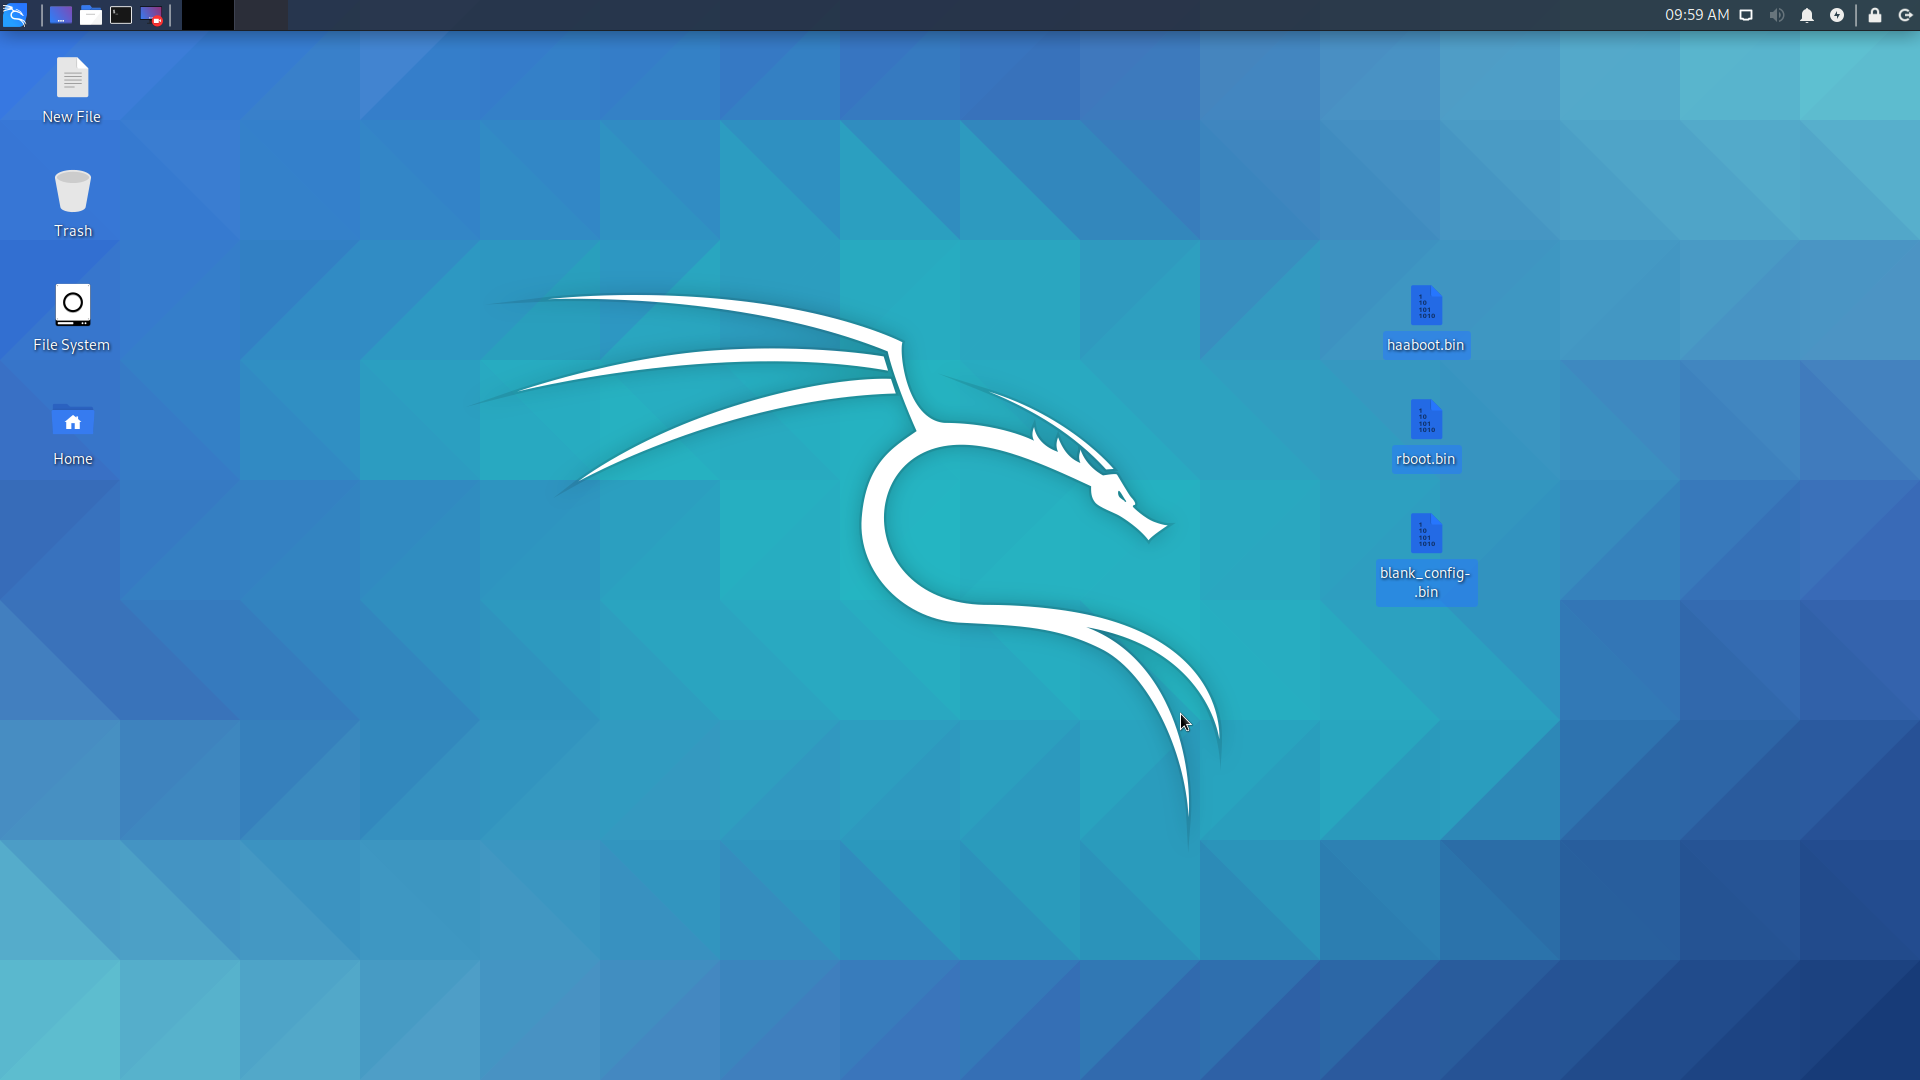
\includegraphics[width=\textwidth]{bin}
	\caption[bin]{所需所有的二进制文件}
	\labfig{normalbin}
\end{figure*}


\pagelayout{wide} % No margins
\addpart{烧录、配置与部署}
\pagelayout{margin} % Restore margins

\setchapterpreamble[u]{\margintoc}
\chapter{固件烧录与配置}
\labch{flandco}

\setlength\parindent{2em} 上一章中,适用于本项目的操作系统与应用程式的编译与准备已经完成,本章将介绍将操作系统与应用程式的二进制文件烧录到单片机上的过程,并将其配置到合适状态的过程。本章最后会将整个开关电路组装并且进行试验,为下一章的电路部署做准备。

\section{固件的准备与烧录}

\setlength\parindent{2em} 上一章中已经将所需的操作系统与应用程式进行选择与编译,最终得到三个二进制文件。下一步,将三个二进制文件合成一个,暂且称之为一个完整的“固件”——即写入可擦写可编程只读存储器中的程序。它的一部分十六进制编码大致如下:\reffig{normalhex}

\begin{figure*}[h!]
	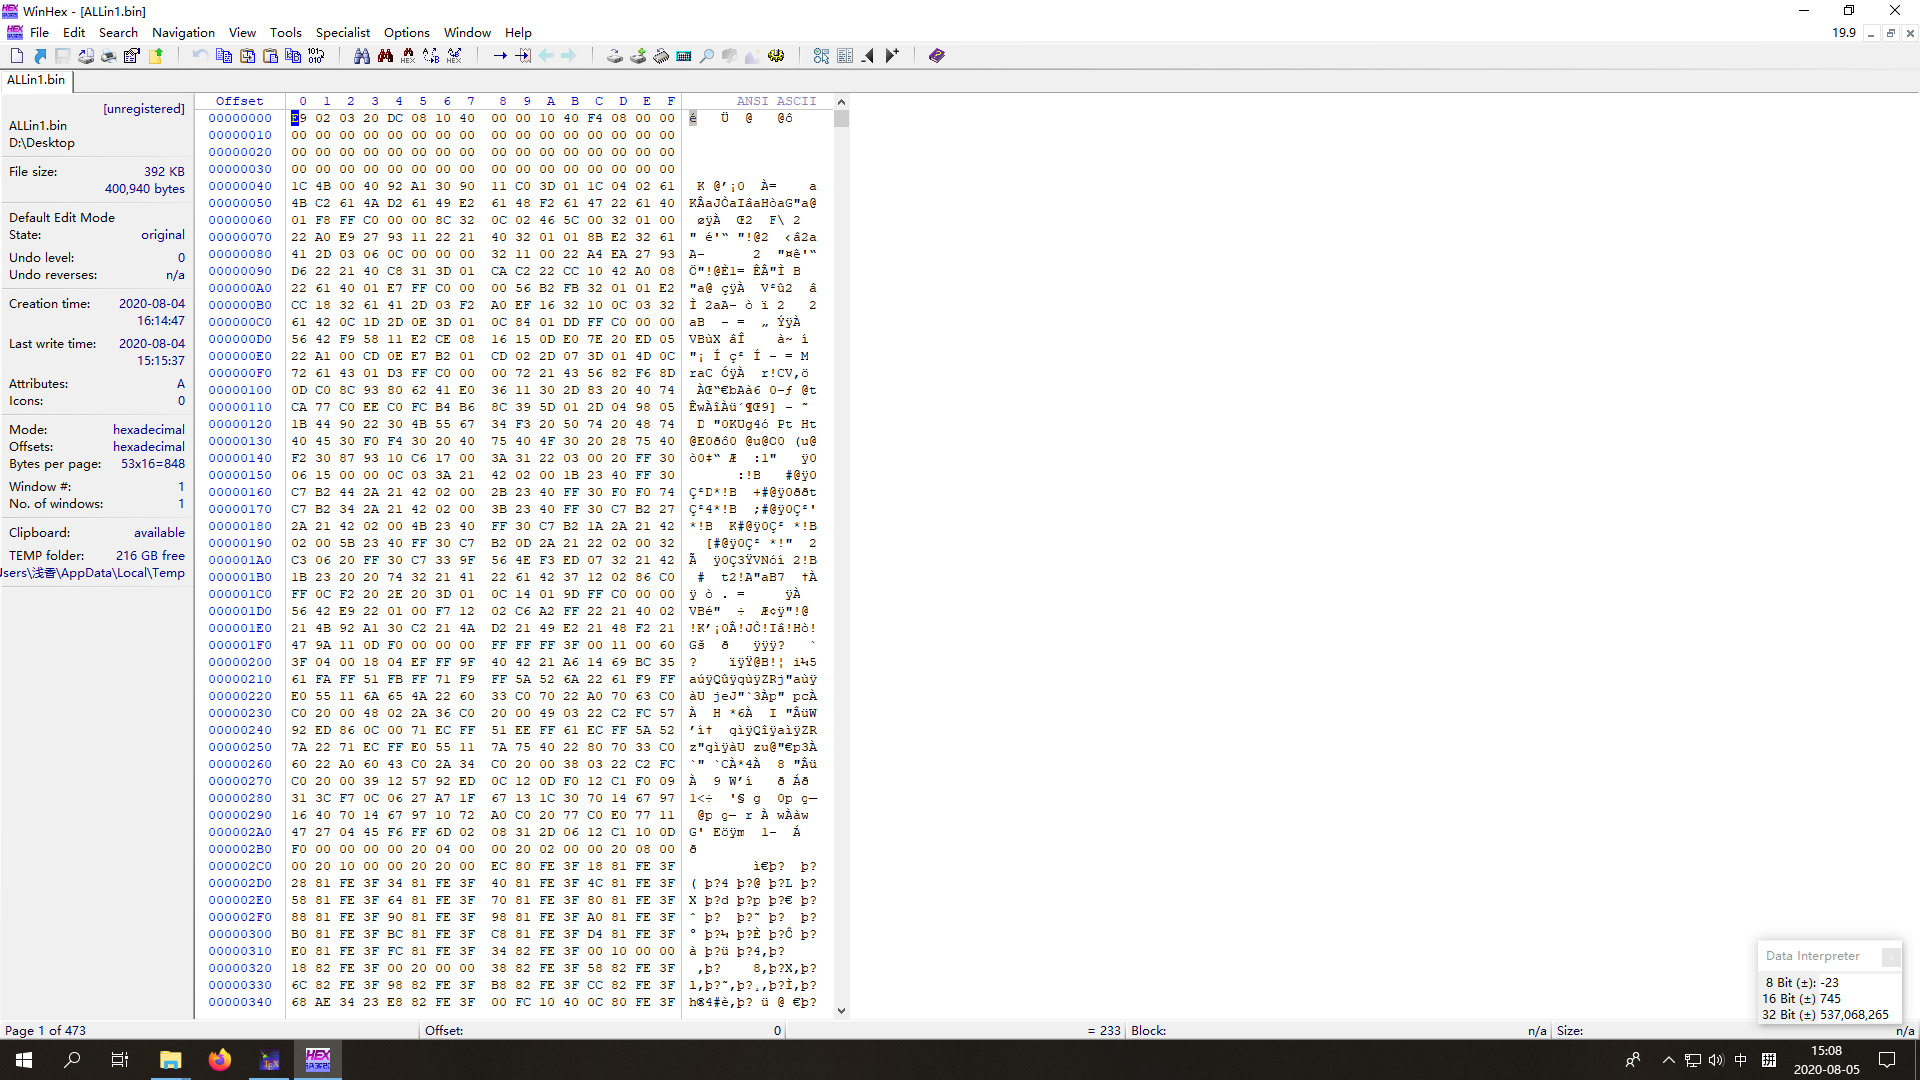
\includegraphics[width=\textwidth]{hex}
	\caption[hex]{固件的十六进制编码的一部分}
	\labfig{normalhex}
\end{figure*}

\par 固件已经准备完成,下一步就是把它烧录的微控单元中,即将其写入微控单元的储存器。根据Espressif Inc.官方提供的文档,可以下载到适用于ESP芯片的烧录程序\sidenote{\url{https://www.espressif.com/sites/default/files/tools/flash_download_tool_v3.8.5.zip}}。将其下载后,准备UART转换至USB的转换器,以通过通用异步收发传输器\sidenote{通用异步收发传输器(Universal Asynchronous Receiver/Transmitter),通常称作UART,是一种通用串行数据总线,用于异步通信。该总线双向通信,可以实现全双工传输和接收。它将要传输的资料在串行通信与并行通信之间加以转换。作为把并行输入信号转成串行输出信号的芯片,UART通常被集成于其他通讯接口的连结上。}与计算机之间进行串行通信。本次使用的转换器芯片为CP2104,为CP210x类芯片之一,比较常用的串行通信芯片。将其与计算机连接后,运行烧录程序,预先在端口设置中将调制速率调节至115200。在烧录程序中清除微控单元的闪存芯片,填充为0,再将准备好的固件从0x0,即第零扇区开始烧写,整个过程需要几分钟,如图\reffig{normalflash}所示:

\begin{figure*}[h!]
	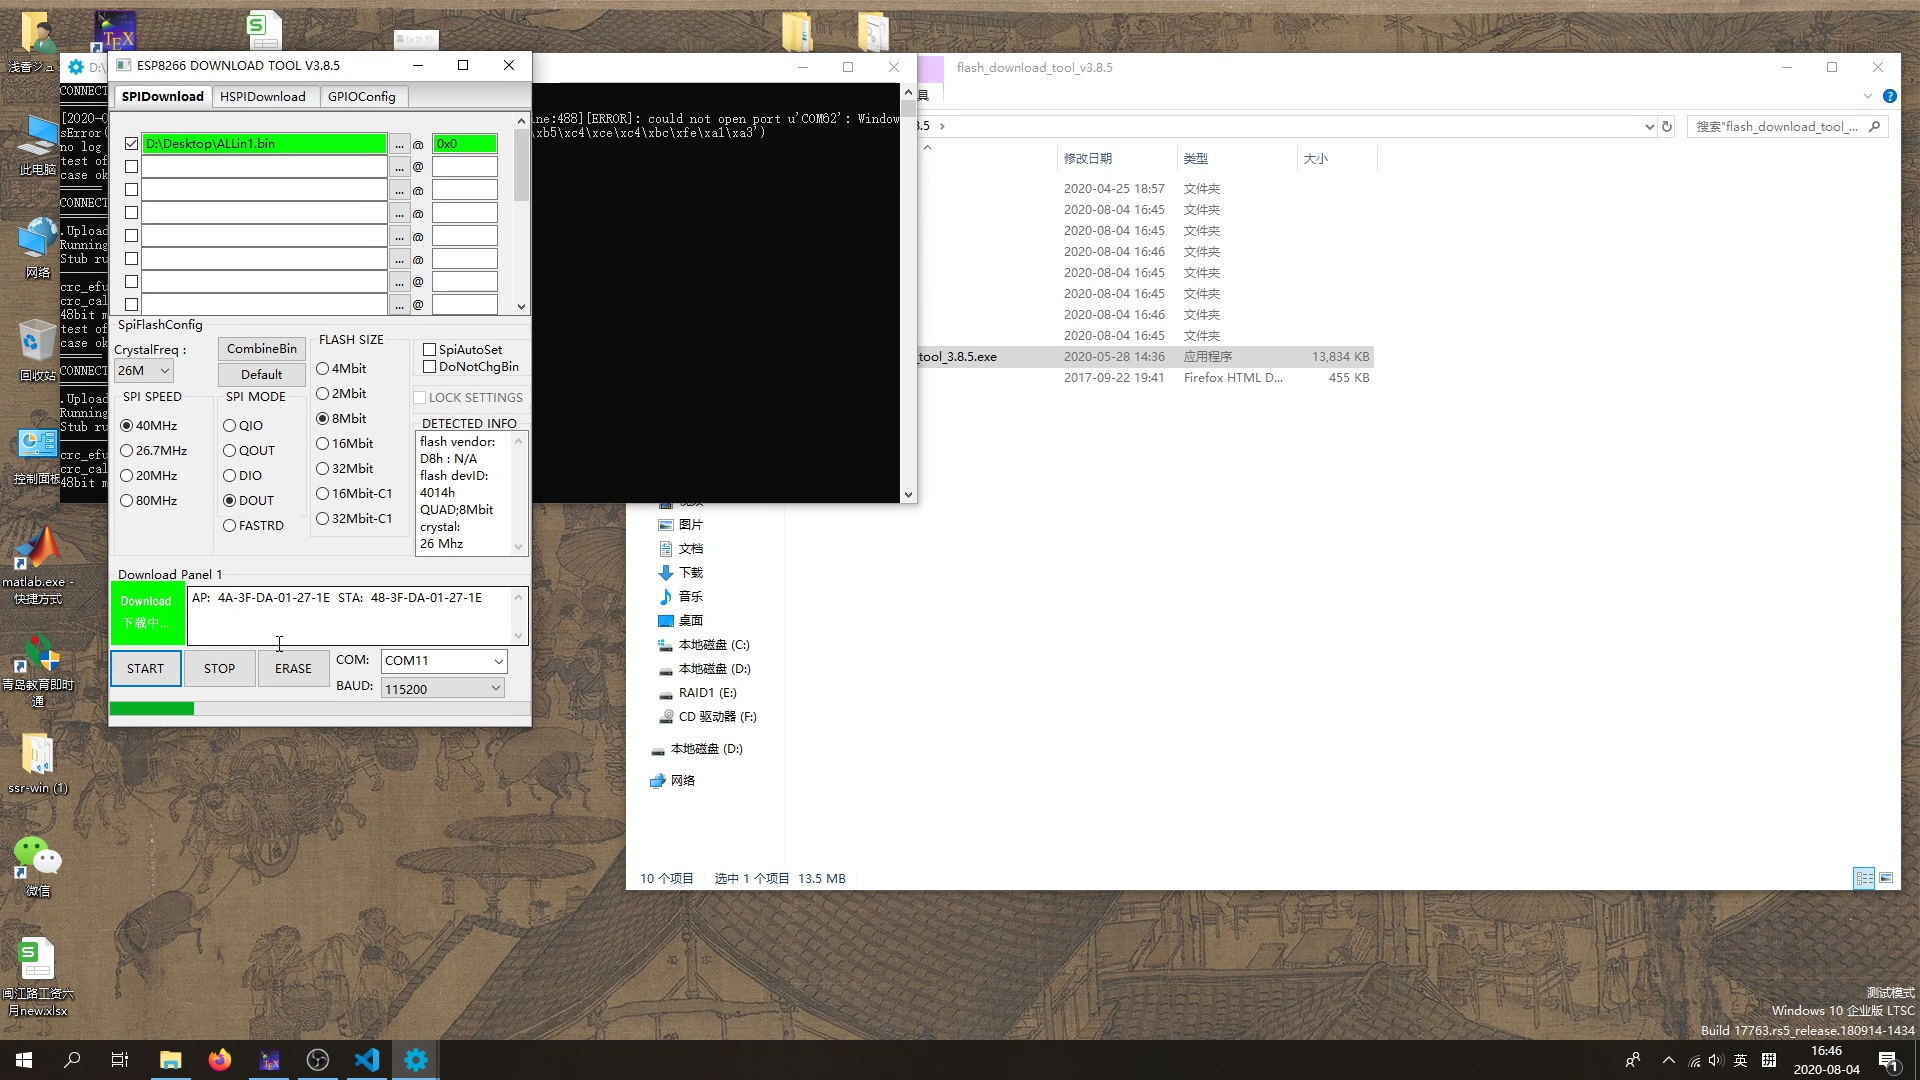
\includegraphics[width=\textwidth]{flash}
	\caption[flash]{固件烧写的过程}
	\labfig{normalflash}
\end{figure*}


\begin{marginfigure}[0cm]
	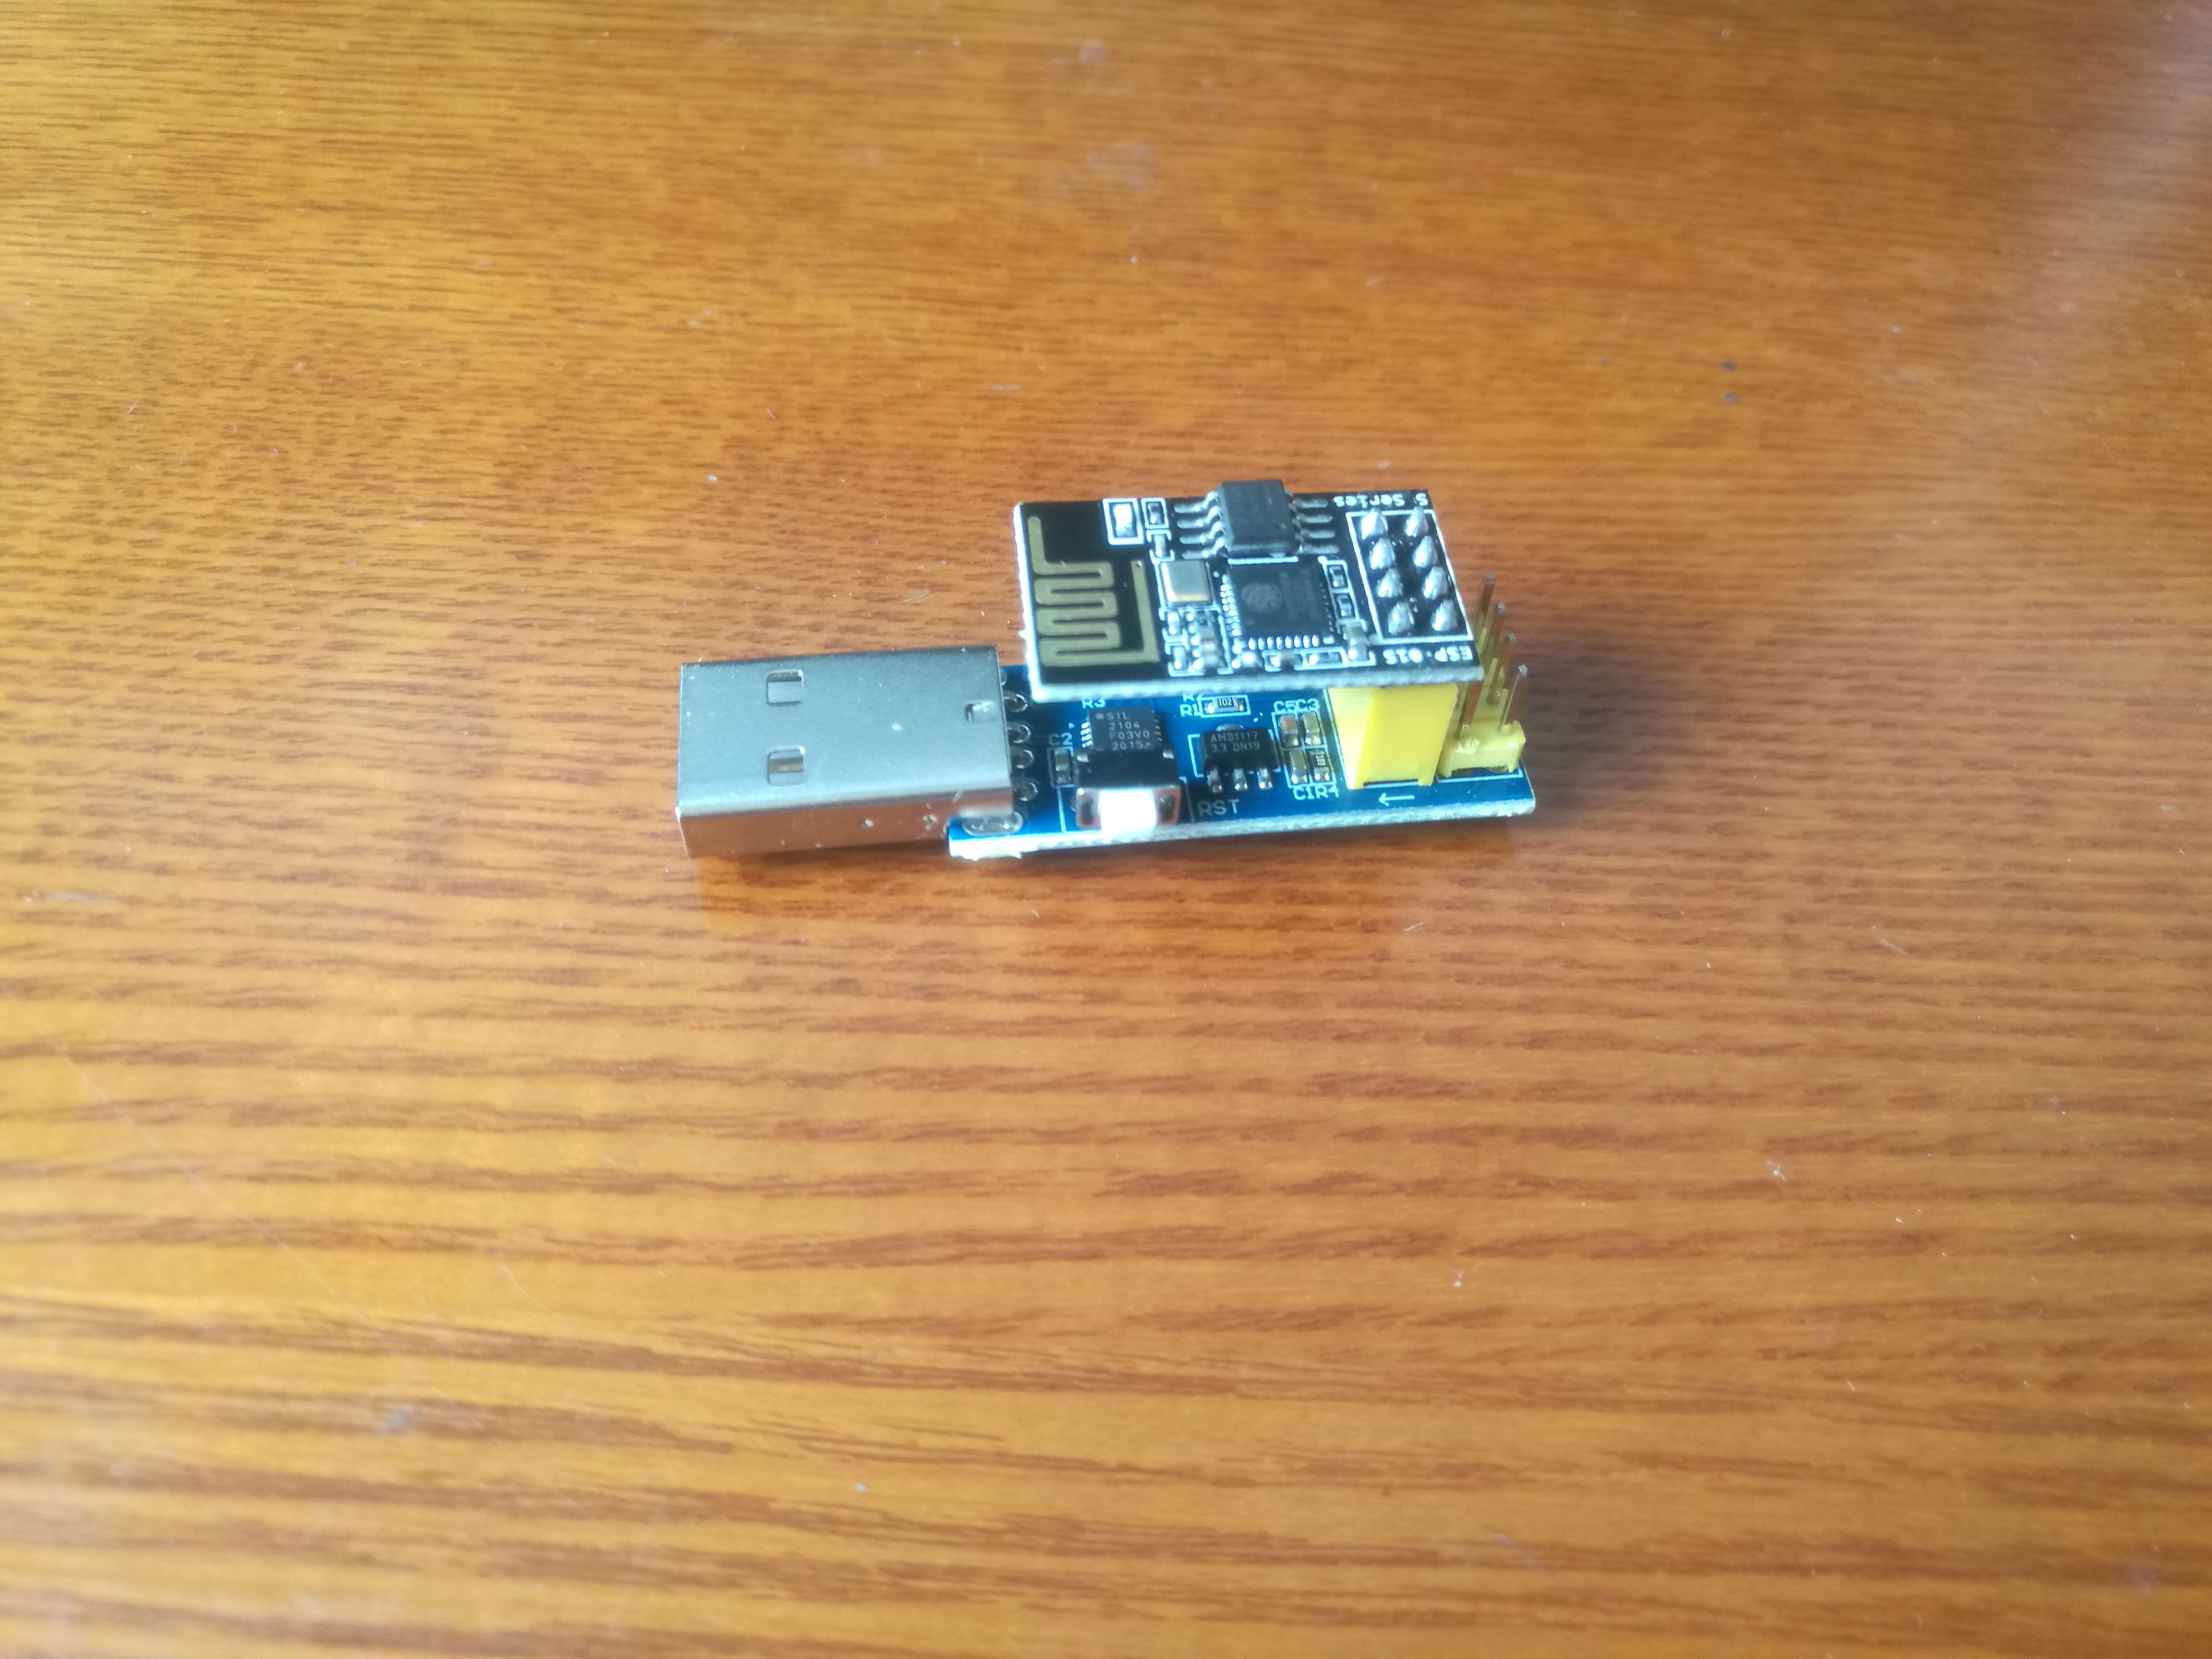
\includegraphics{flasher}
	\caption[flasher]{微控单元与烧写器}
\end{marginfigure}

\par 至此,烧录完成。将微控单元与烧写器断开,将其接至继电器模块上的端口。并且将继电器模块上的供电用端子座连接上5V直流电源,此时继电器应该突然闭合又断开,可以在附近搜索到SSID为HAA开头的Wi-Fi协议无线网络信号,表示烧录成功。

\section{应用程式的配置}

\setlength\parindent{2em} 烧录成功后,进入配置阶段。根据HAA官方位于GitHub上的Wiki,需要编写json来对设备进行配置,或者说是编程;将连接的设备、电平的高低、触发器、指示灯等等进行控制。在硬件电路的设计中,按照最后的设计图,继电器闭合对应着GPIO0的低电平,若GPIO0为高电平,则继电器断开,或者说是公共端与常闭端导通。于是得到如下配置:继电器与GPIO0连接;继电器正常状态为GPIO0的高电平;继电器在电路通电时默认断开。其它按照Wiki中的设置,未作修改。最终完整的json文件如下图\reffig{normaljson}所示:

\begin{figure*}[h!]
	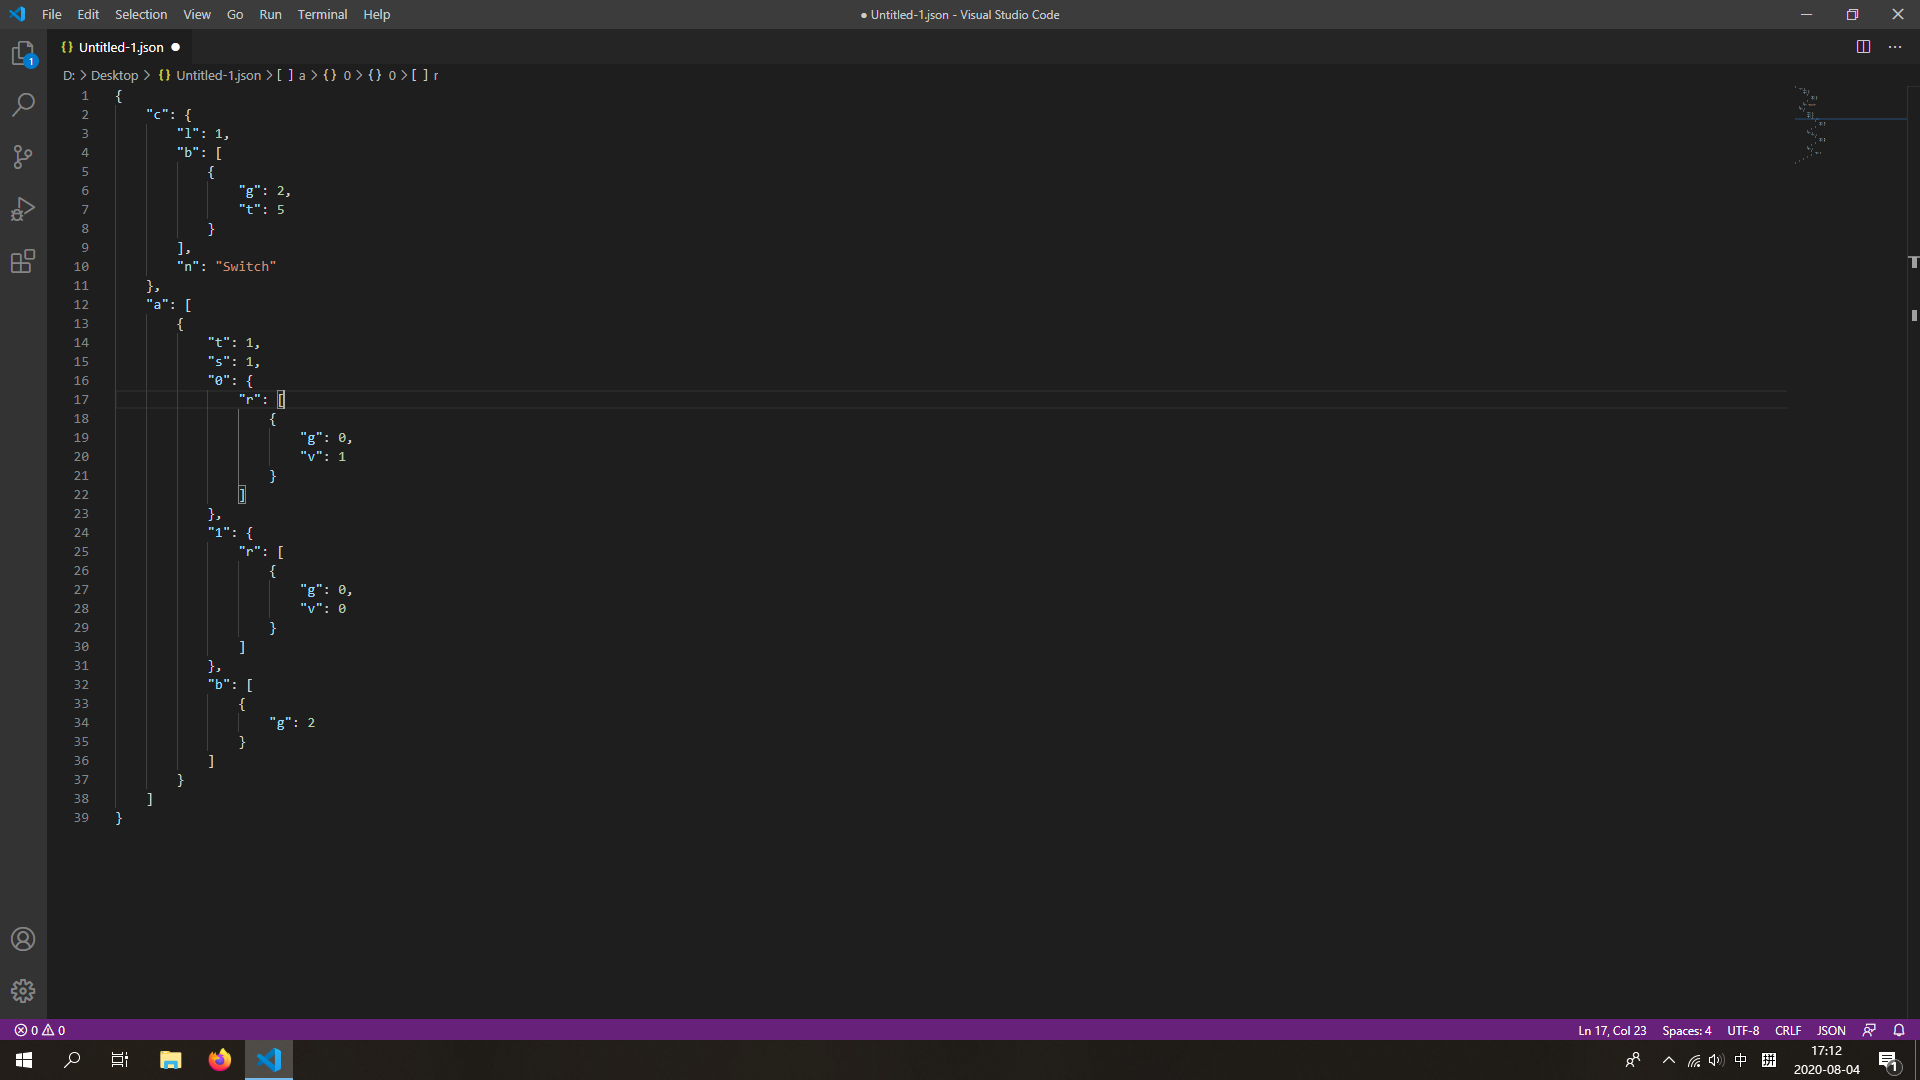
\includegraphics[width=\textwidth]{json}
	\caption[json]{完整的json配置文件}
	\labfig{normaljson}
\end{figure*}

\par 接下来进行设备的配置。将微控单元与继电器模块连接后,模块上的端子座通上5V直流电,此时可以在附近搜索到没有加密的Wi-Fi协议无线网络。加入无线网路,用浏览器访问http://192.168.4.1/,这个网址可以在HAA的Wiki上找到,以为本设备,为这个应用程式的配置页面。进入后如图\reffig{normalconf}所示:

\begin{figure*}[h!]
	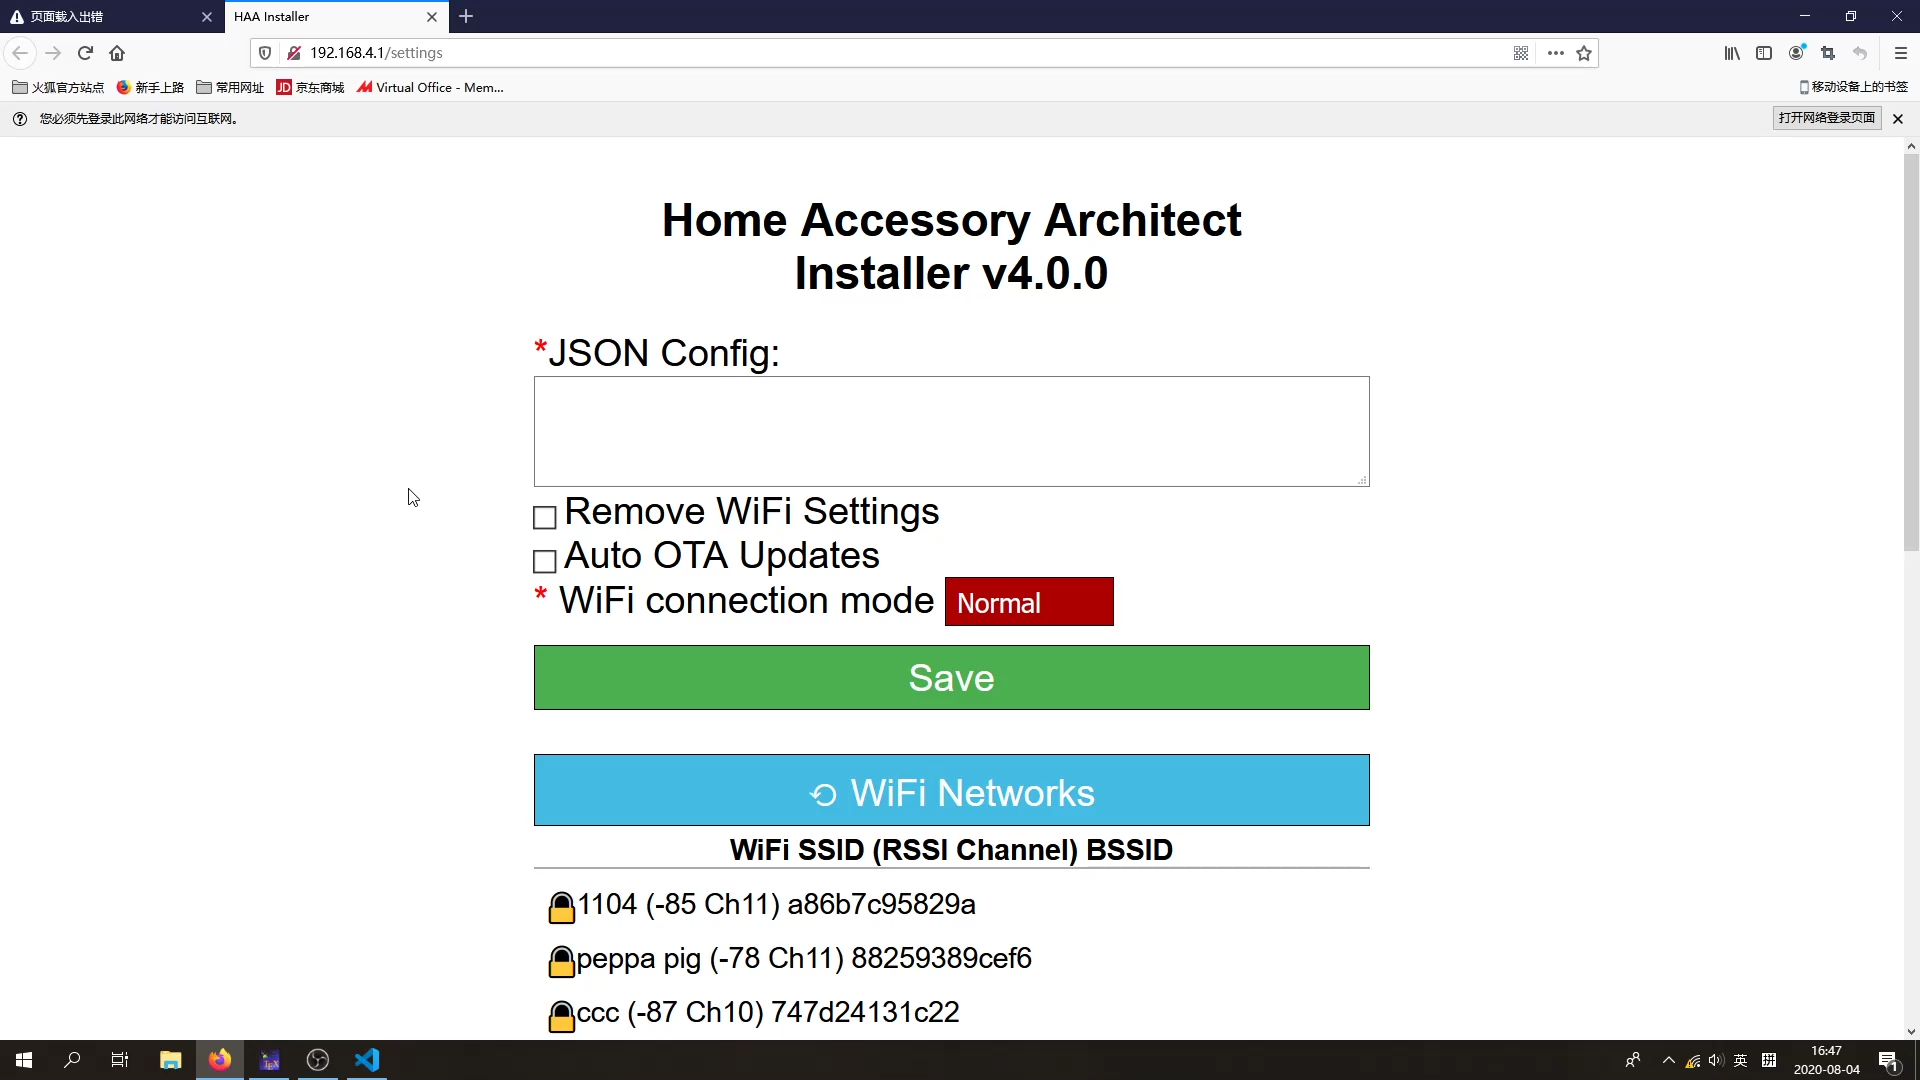
\includegraphics[width=\textwidth]{conf}
	\caption[conf]{微控单元应用程式的配置页面}
	\labfig{normalconf}
\end{figure*}

\par 接下来就很简单,将json配置填写到顶部JSON Config一栏,最好将json格式化为一行,这样可以节省对储存器的占用——根据官方Wiki所说。在下面选择所要连接的无线网络(仅支持Wi-Fi协议),输入密码,点击Save,配置就完成了。

\par 然后就需要等待了。由于微控单元的处理能力极为低下,所以其将配置应用到设备并接入无线网络所用的时间相对较长,大概需要十多分钟才可以进行下一步的连接。当其配置完成后,微控单元上的LED指示灯应该会闪烁一下。

\begin{marginfigure}[0cm]
	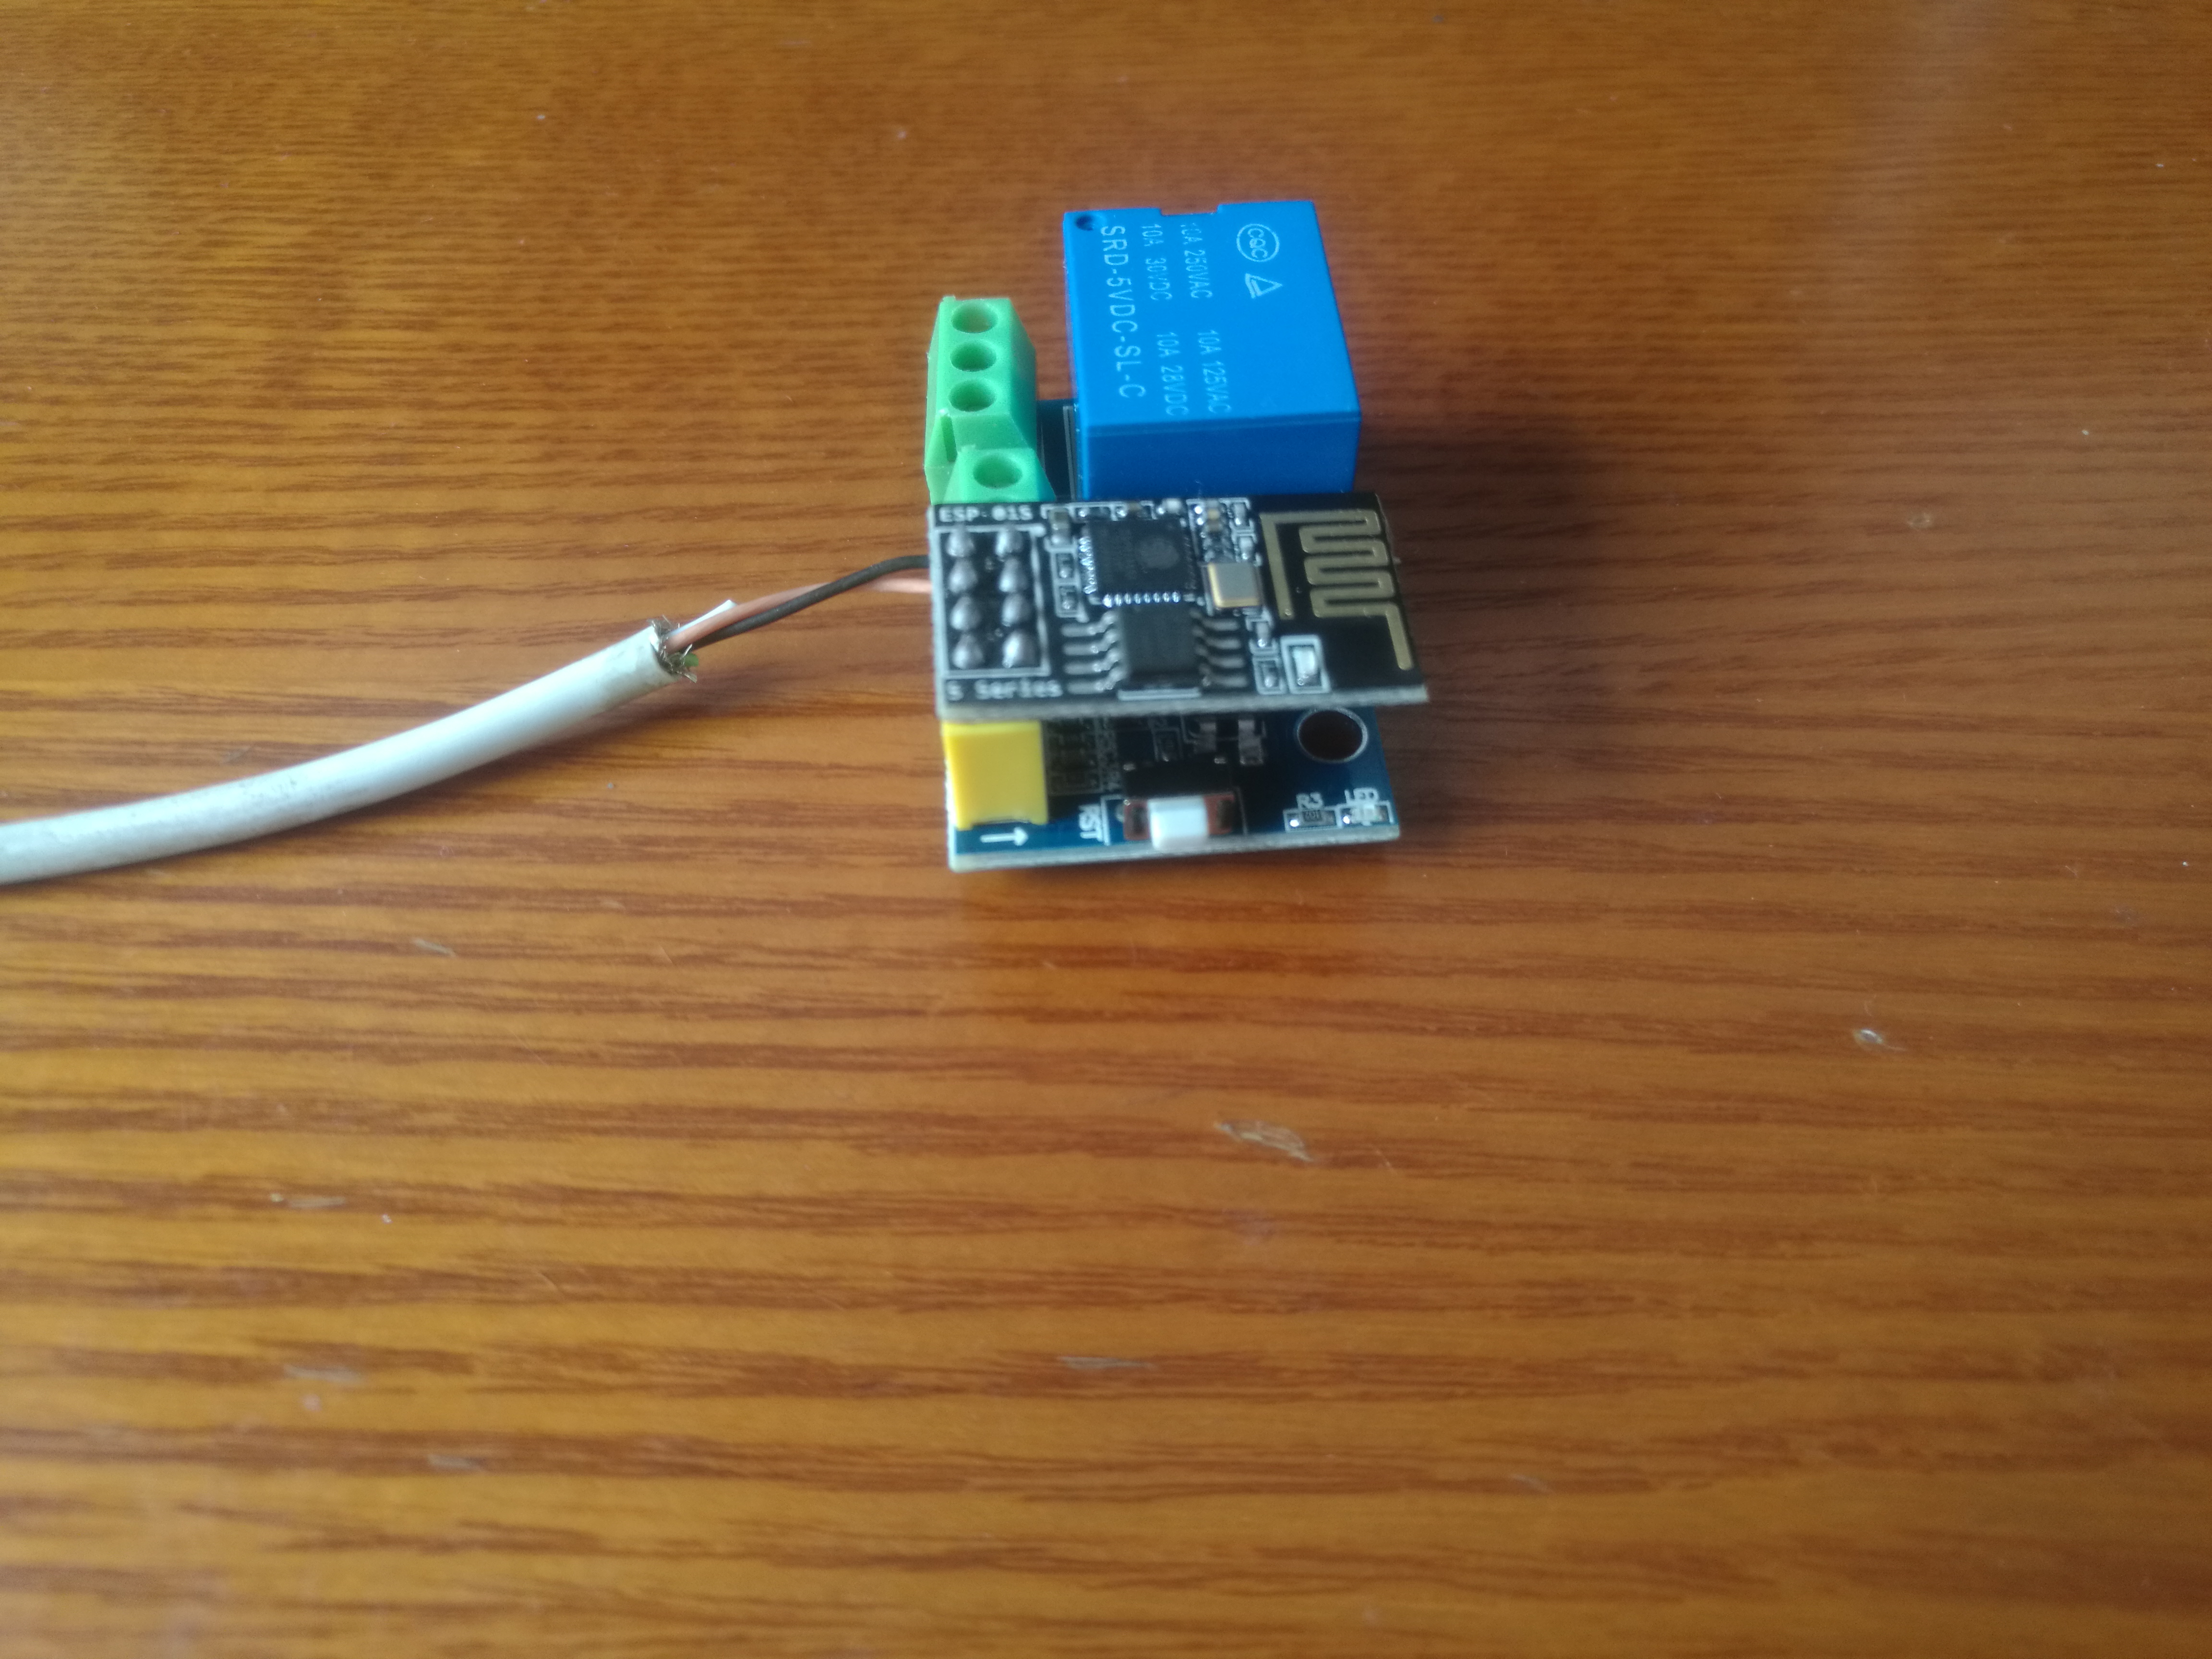
\includegraphics{all}
	\caption[all]{微控单元与继电器}
\end{marginfigure}

\section{继电器电路与客户端的连接}

\setlength\parindent{2em} 应用程式配置好后等待其自动应用配置,然后即可与Apple HoneKit客户端进行连接。按照Apple Inc.官方开发文档,对开发与调试描述地很详细,在此要做的就是将微控单元与Apple智能设备连接到同一无线网络下,上一节已经将微控单元接入网络。此时,打开Apple智能设备中的“Home”应用程序,非特殊情况,仅支持运行iOS8及以上的Apple设备。点击“Add Accessory”。由于没有提供可供扫描的QR二维码,选择“Don't Have a Code”,此时一个名为HAA开头的设备应该出现在屏幕上。根据HAA官方Wiki,所有的HAA应用程式所用的连接代码是一样的。如图\reffig{normalcode}所示。

\begin{marginfigure}[0cm]
	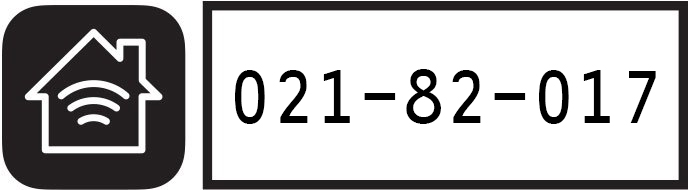
\includegraphics{code}
	\caption[code]{连接代码}
	\labfig{normalcode}
\end{marginfigure}

\par 输入代码后,会自动连接,大概需要一分多钟。连接后,如图\reffig{normalresult}所示,即可自由控制该继电器,继电器模块上的LED表示继电器的状态,若灯亮则表示继电器导通(公共端与常闭端导通);反之,则公共端与常开端导通。若测试有效,则表明电路正常工作,可以进行下一步的电路部署工作了。

\begin{figure*}[h!]
	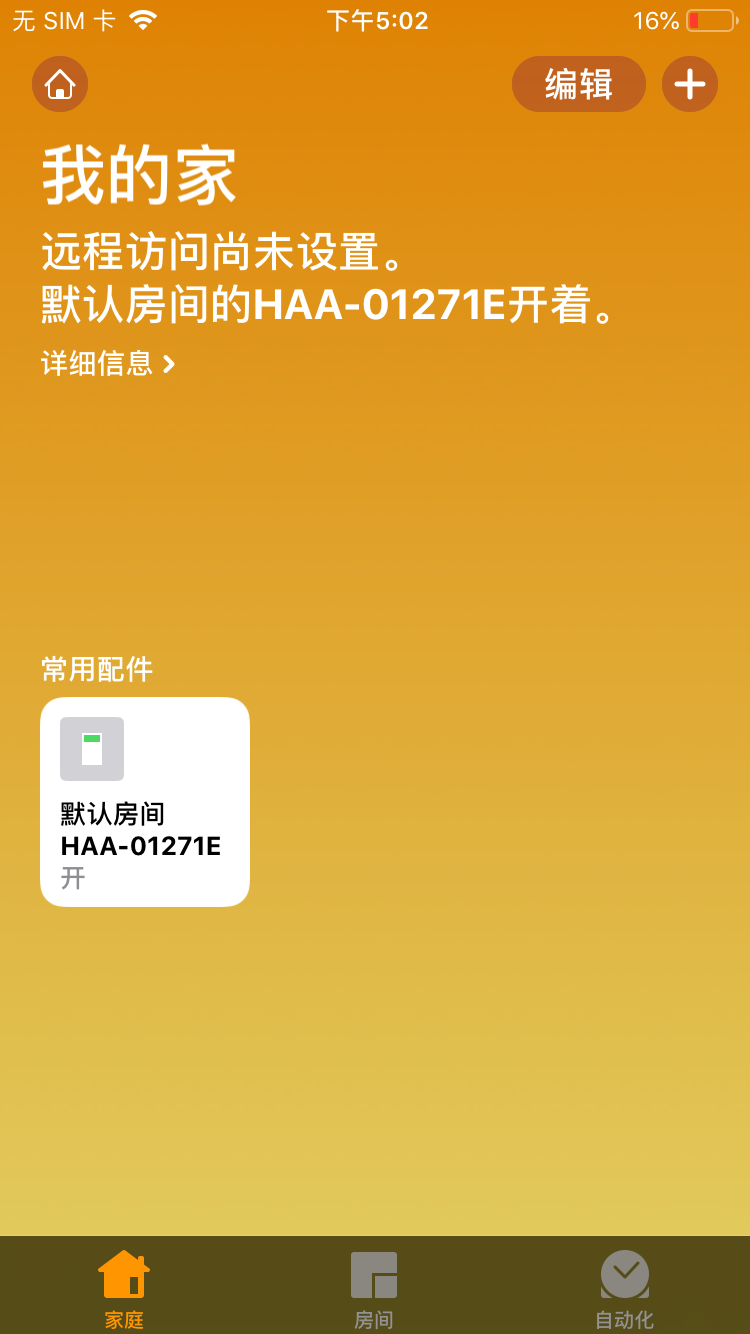
\includegraphics[width=\textwidth]{result}
	\caption[result]{连接成功}
	\labfig{normalresult}
\end{figure*}

\setchapterpreamble[u]{\margintoc}
\chapter{电路部署}
\labch{deploy}

\setlength\parindent{2em} 本章将进行电路的部署,即将继电器电路与生活用电器连接。本次选择了讲述方便、便于演示、功率小,安全性高的台灯最为演示用案例。最终将其部署成一个联网、智能化的台灯。

\section{电路规划}

\setlength\parindent{2em} 原台灯的电路简图如图\reffig{normallightori}所示。原台灯中已经有一个开关,位于火线上、镇流器之前,直接控制220V的通断。本次想要形成的效果是:两个开关分别独立,两个开关同时断开时,电路开路;否则电路为通路。换句话说,假设继电器与开关分别为A、B,则电路的通断状态R = A || B。

\begin{figure*}[h!]
	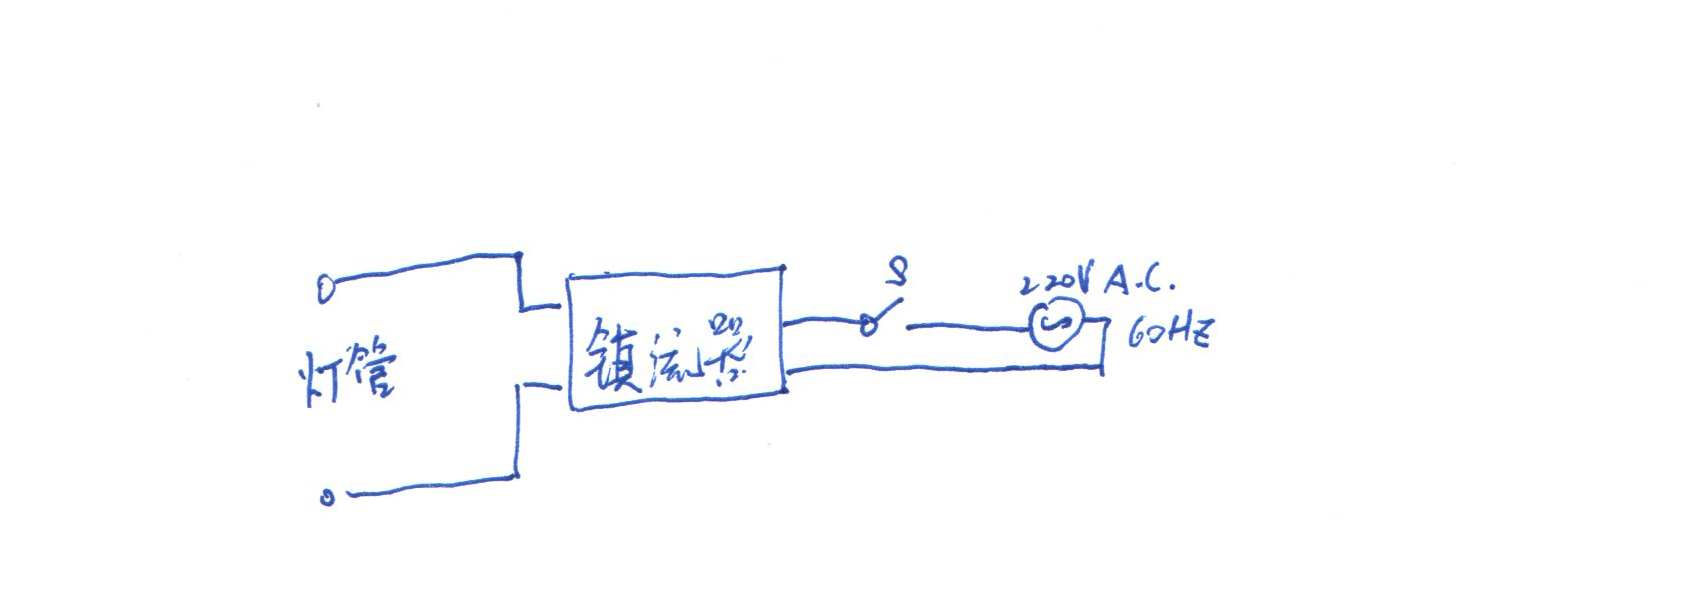
\includegraphics[width=\textwidth]{lightori}
	\caption[lightori]{原台灯的电路图}
	\labfig{normallightori}
\end{figure*}

\par 为实现此目的,需要将开关与继电器并联,最终形成的电路图如图\reffig{normallight}所示。继电器与开关并联,同时置于火线上。继电器的5V供电通过USB接口单独引出,利用220V AC-5V DC的降压模块供电。最终整个电路即可完成。

\begin{figure*}[h!]
	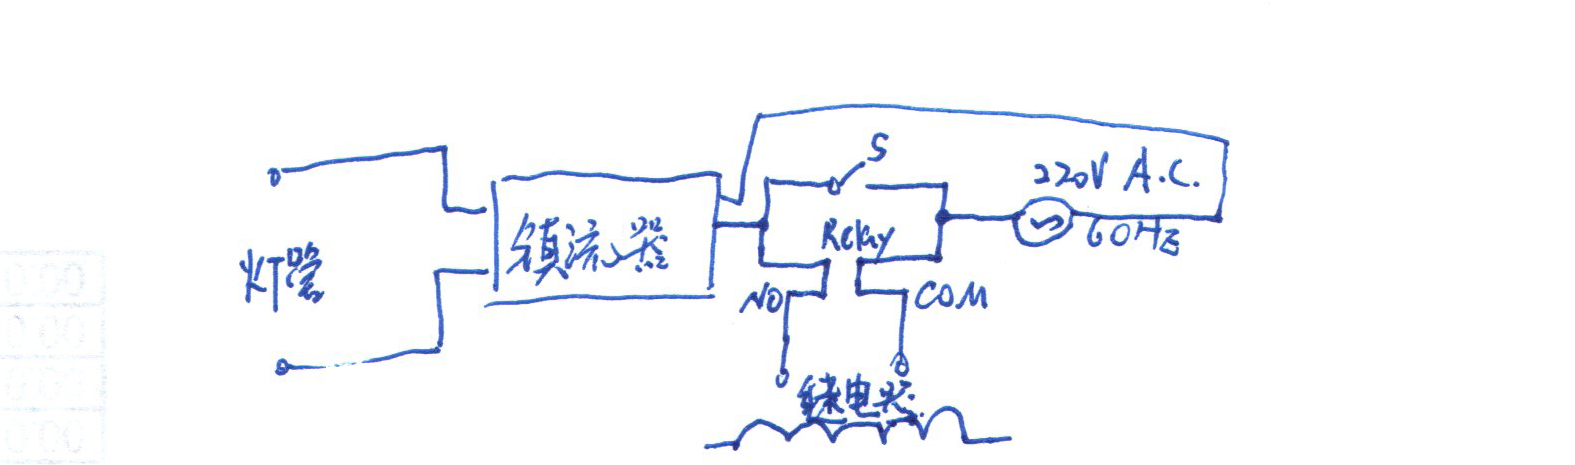
\includegraphics[width=\textwidth]{light}
	\caption[light]{部署后台灯的电路图}
	\labfig{normallight}
\end{figure*}

\section{成果展示}
\setlength\parindent{2em} 实验效果如下所示:

\begin{figure*}[h!]
	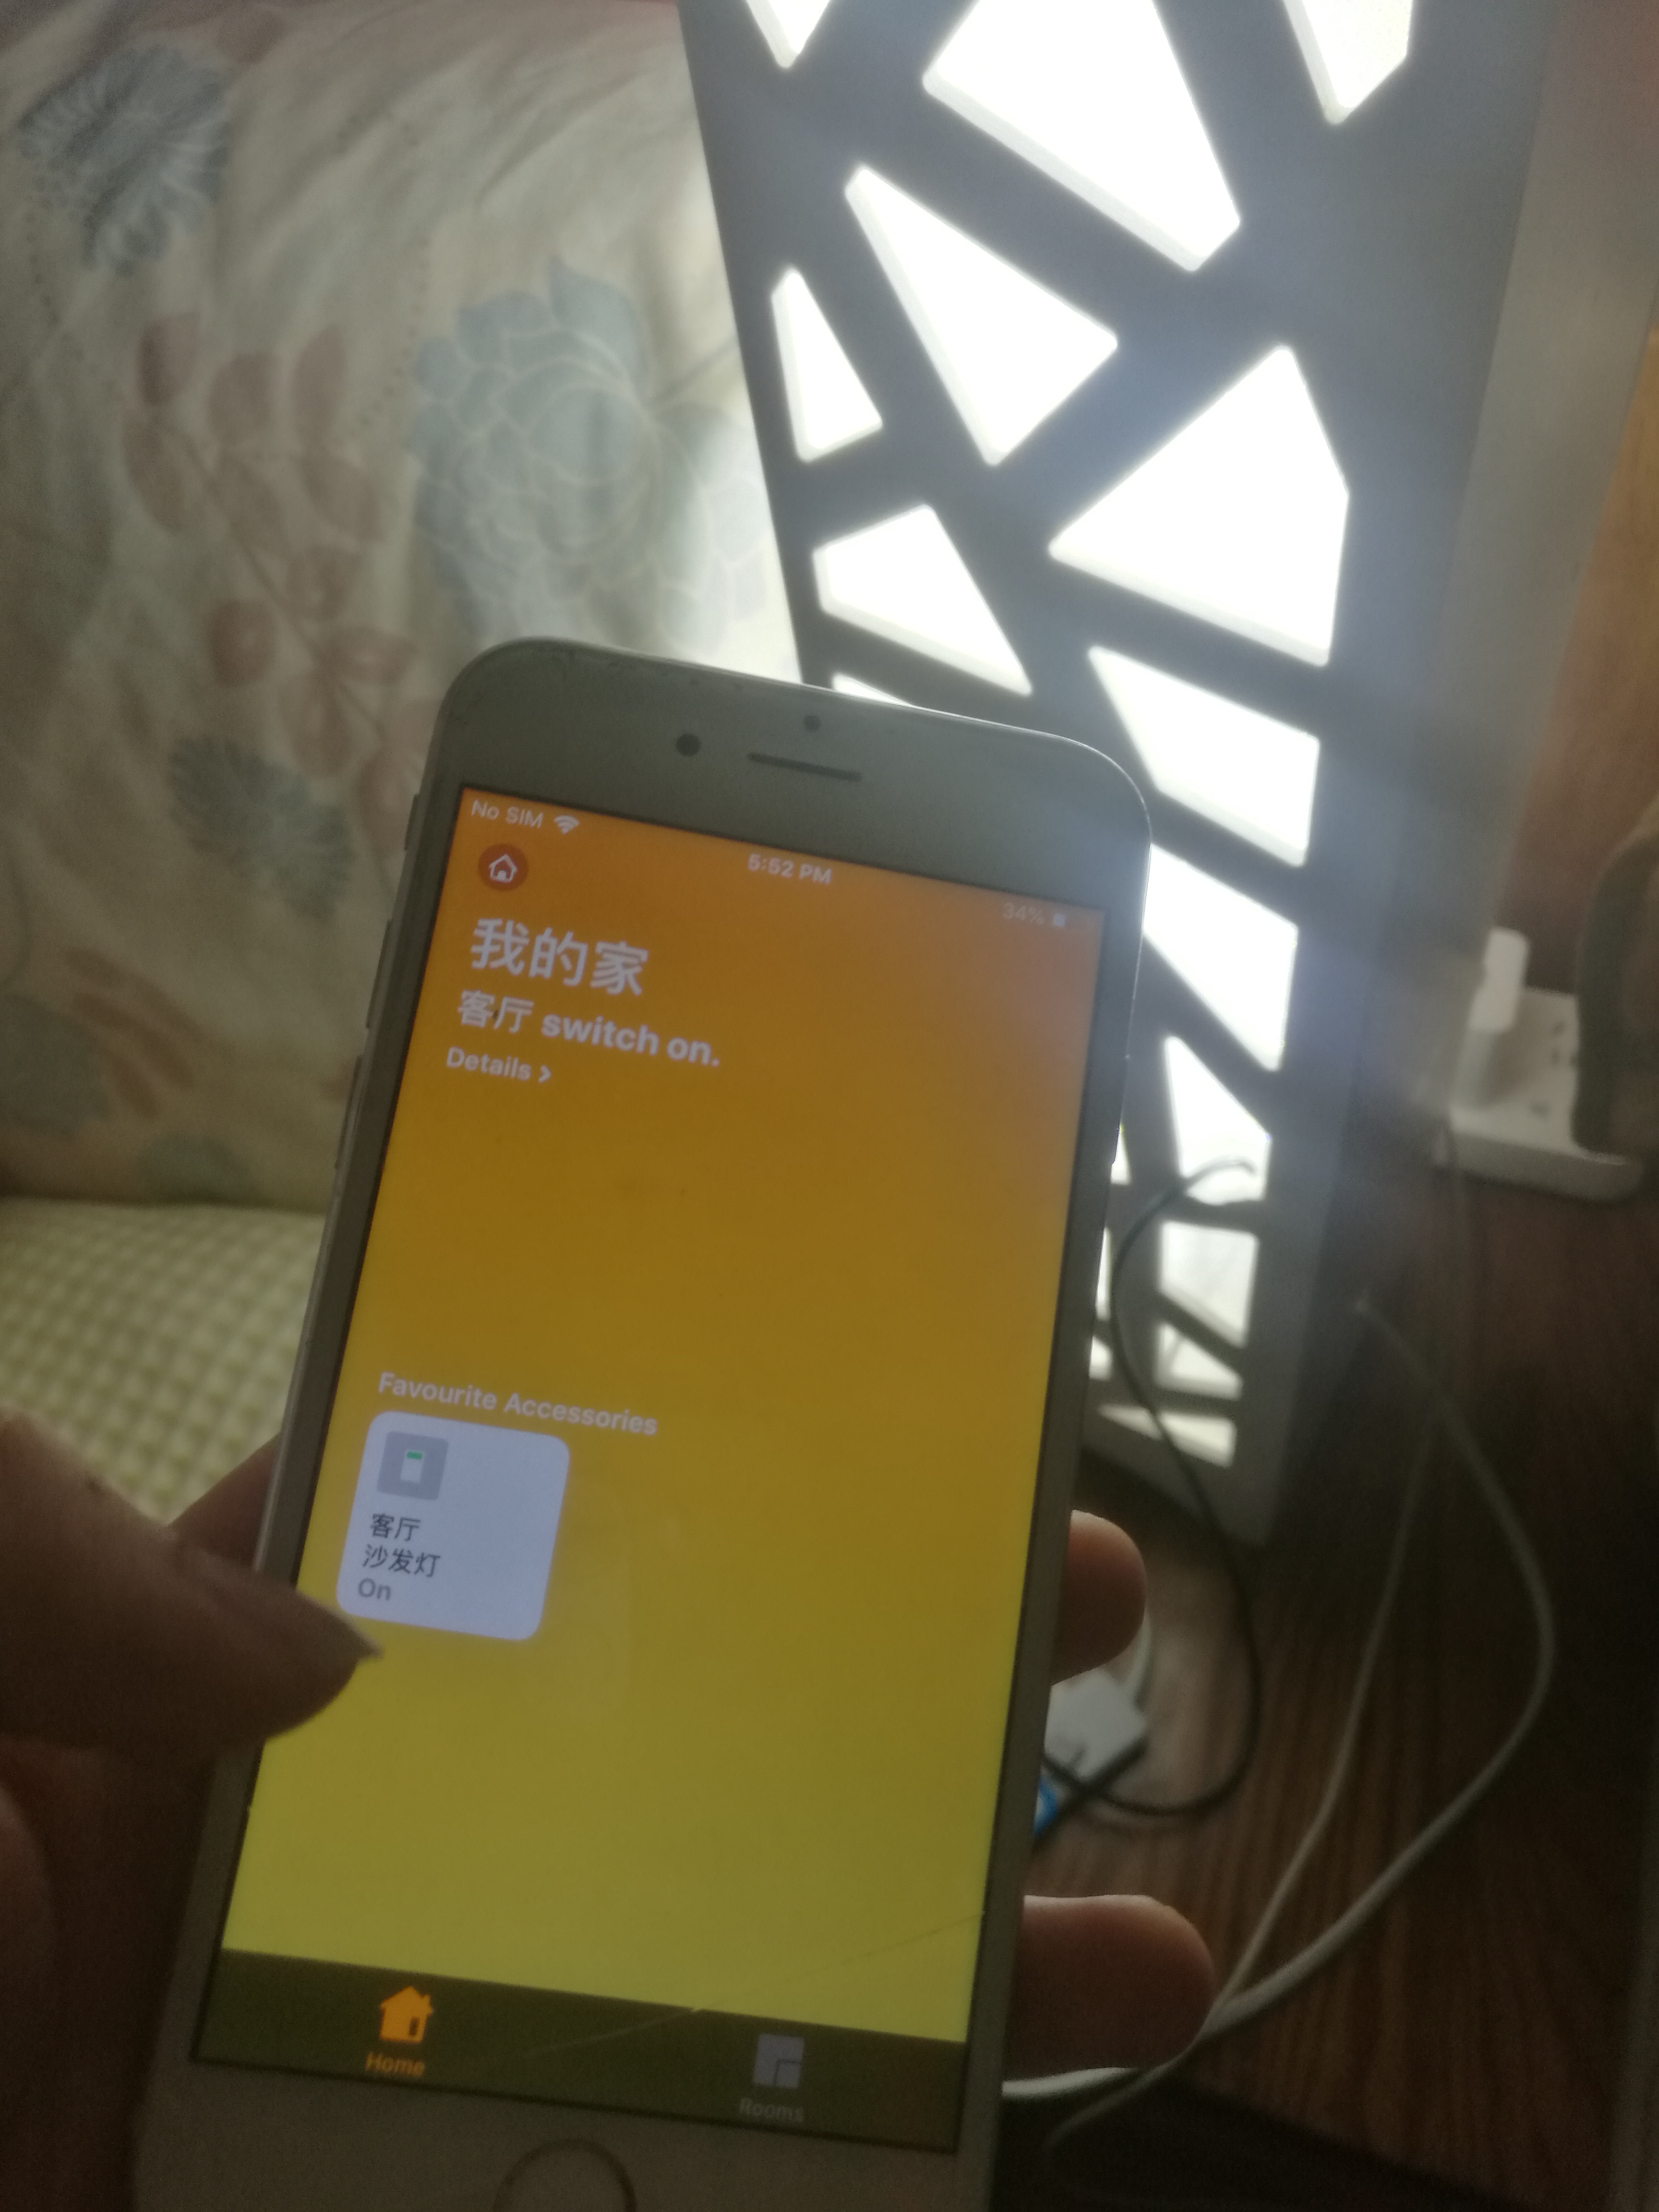
\includegraphics[width=\textwidth]{res}
	\caption[res]{效果图1}
\end{figure*}

\begin{figure*}[h!]
	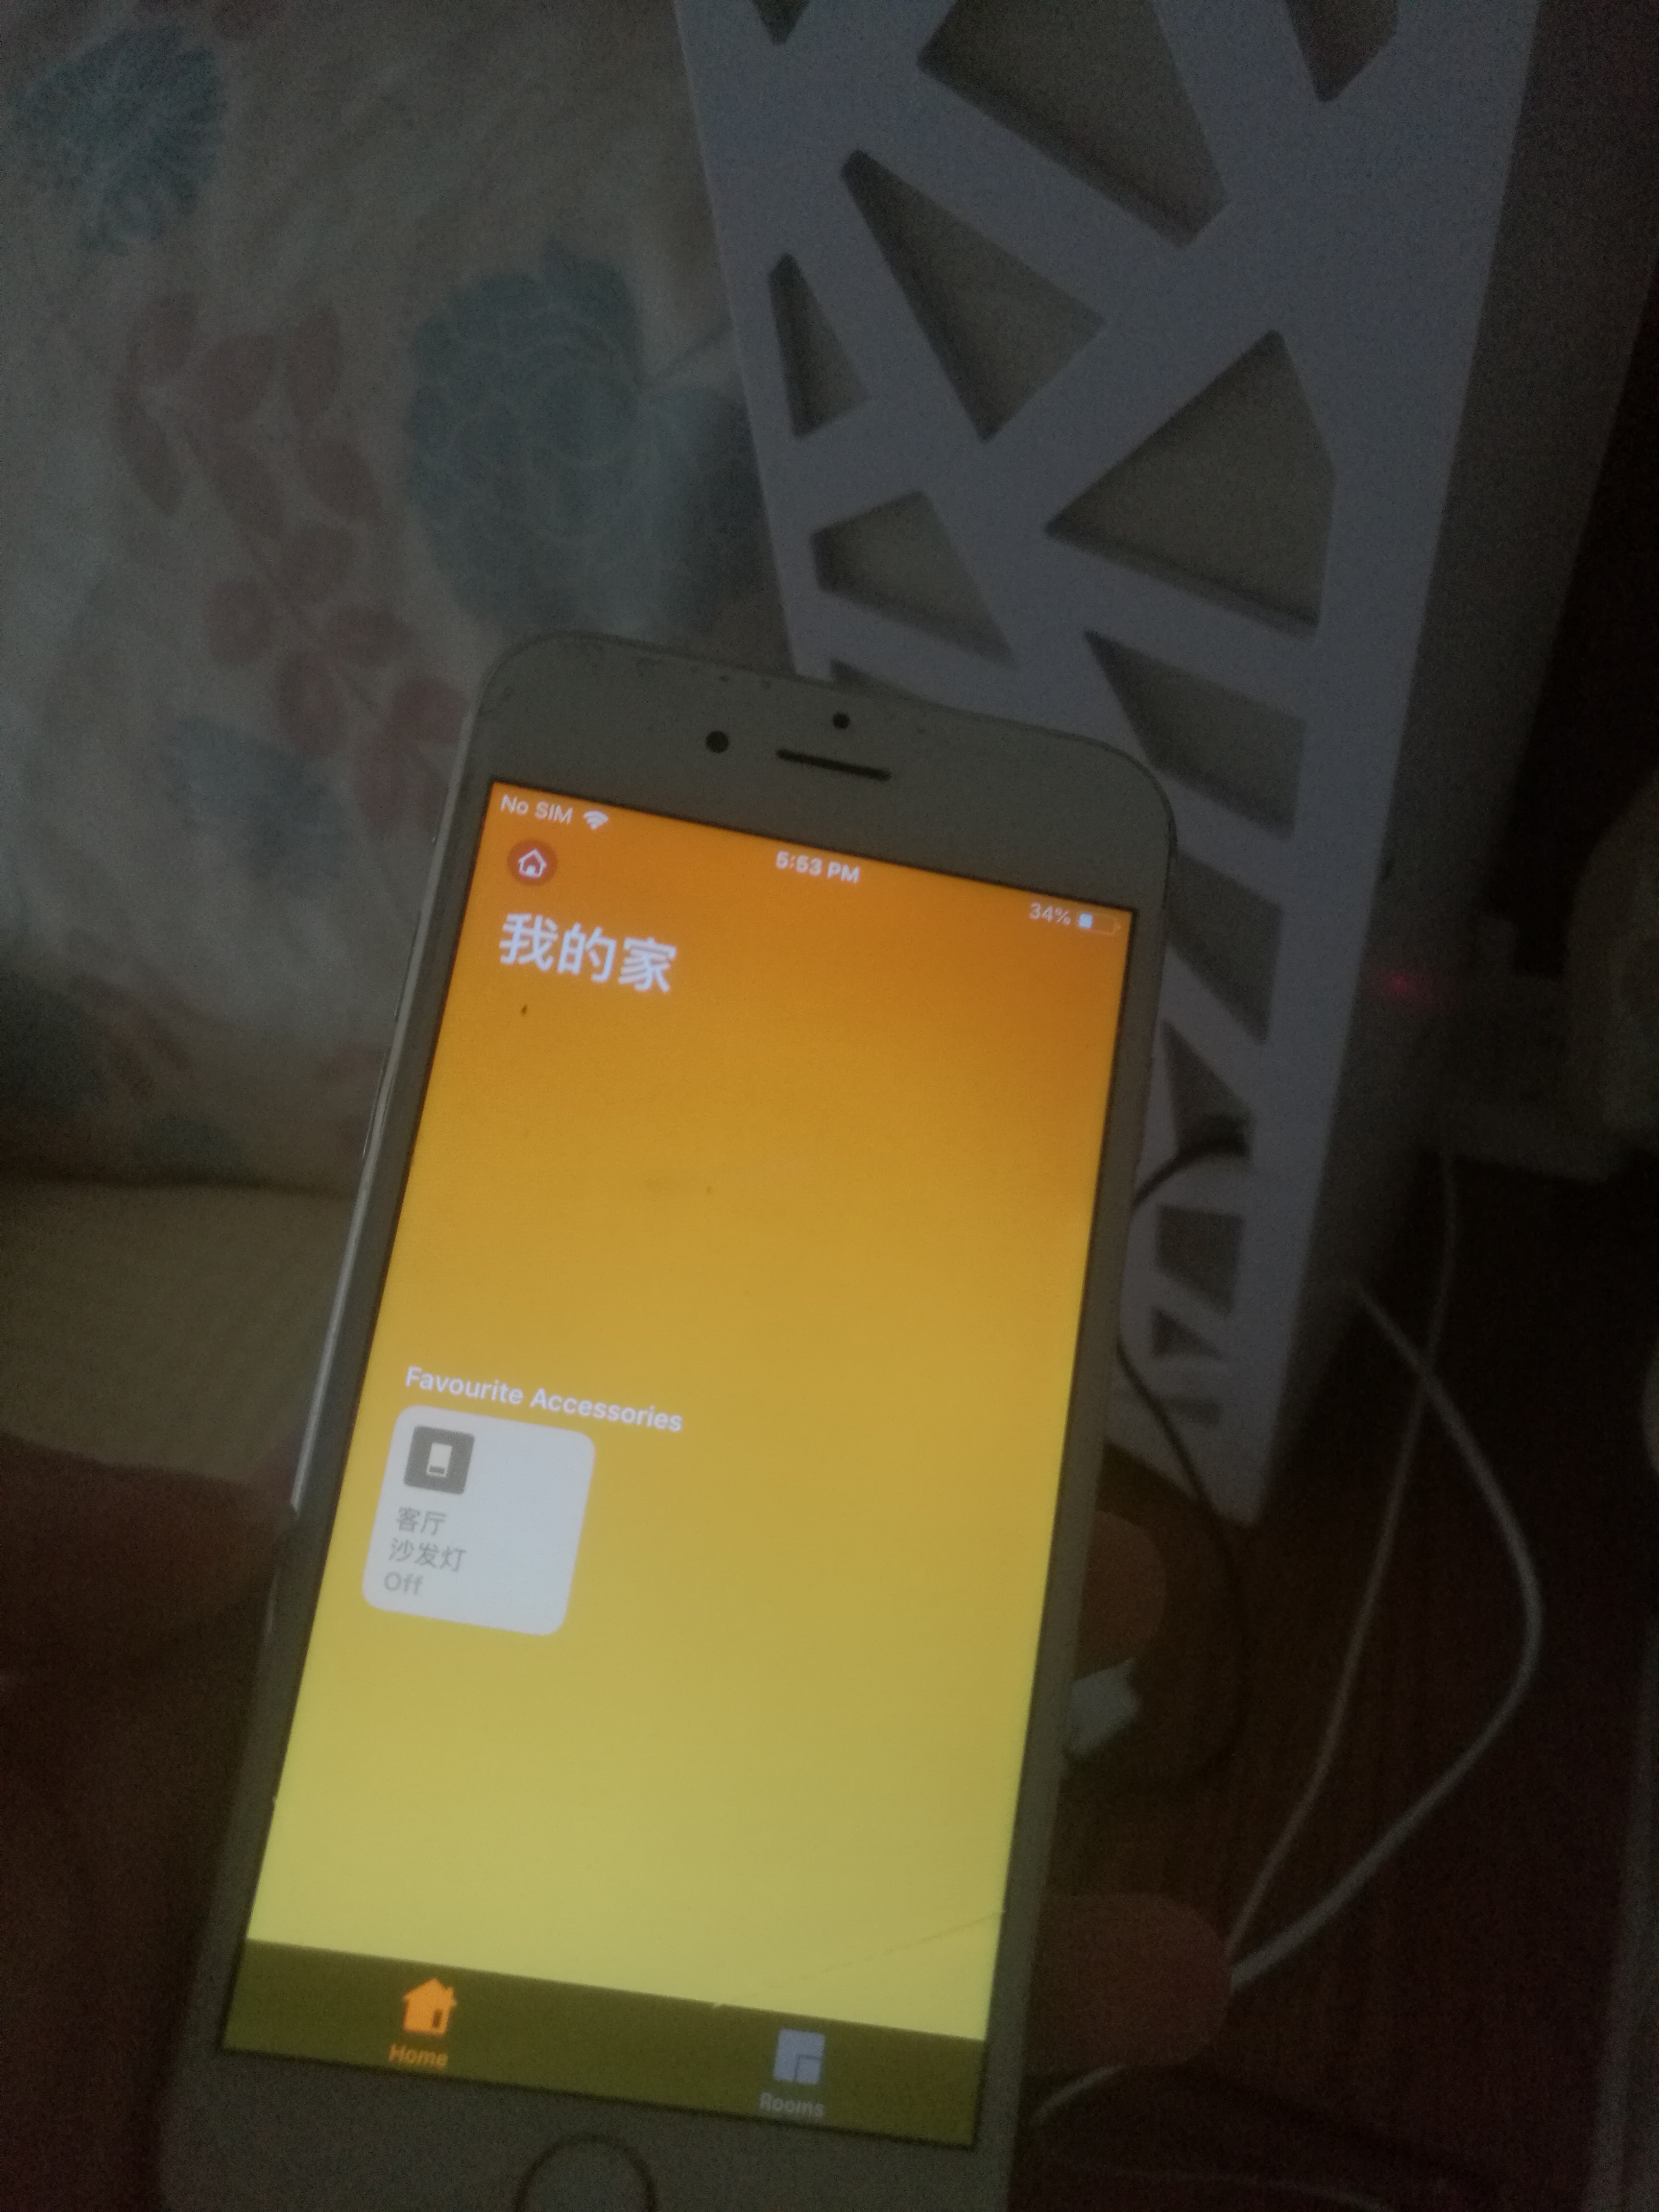
\includegraphics[width=\textwidth]{res1}
	\caption[res1]{效果图2}
\end{figure*}


\appendix % From here onwards, chapters are numbered with letters, as is the appendix convention

\pagelayout{wide} % No margins
\pagelayout{margin} % Restore margins


%----------------------------------------------------------------------------------------

\backmatter % Denotes the end of the main document content
\setchapterstyle{plain} % Output plain chapters from this point onwards

%----------------------------------------------------------------------------------------
%	BIBLIOGRAPHY
%----------------------------------------------------------------------------------------

% The bibliography needs to be compiled with biber using your LaTeX editor, or on the command line with 'biber main' from the template directory

\defbibnote{bibnote}{Here are the references in citation order.\par\bigskip} % Prepend this text to the bibliography
\printbibliography[heading=bibintoc, title=Bibliography, prenote=bibnote] % Add the bibliography heading to the ToC, set the title of the bibliography and output the bibliography note

%----------------------------------------------------------------------------------------
%	NOMENCLATURE
%----------------------------------------------------------------------------------------

% The nomenclature needs to be compiled on the command line with 'makeindex main.nlo -s nomencl.ist -o main.nls' from the template directory

\nomenclature{$c$}{Speed of light in a vacuum inertial frame}
\nomenclature{$h$}{Planck constant}

\renewcommand{\nomname}{Notation} % Rename the default 'Nomenclature'
\renewcommand{\nompreamble}{The next list describes several symbols that will be later used within the body of the document.} % Prepend this text to the nomenclature

\printnomenclature % Output the nomenclature

%----------------------------------------------------------------------------------------
%	GREEK ALPHABET
% 	Originally from https://gitlab.com/jim.hefferon/linear-algebra
%----------------------------------------------------------------------------------------

\vspace{1cm}

%----------------------------------------------------------------------------------------
%	GLOSSARY
%----------------------------------------------------------------------------------------

% The glossary needs to be compiled on the command line with 'makeglossaries main' from the template directory

\newglossaryentry{computer}{
	name=computer,
	description={is a programmable machine that receives input, stores and manipulates data, and provides output in a useful format}
}

% Glossary entries (used in text with e.g. \acrfull{fpsLabel} or \acrshort{fpsLabel})
\newacronym[longplural={Frames per Second}]{fpsLabel}{FPS}{Frame per Second}
\newacronym[longplural={Tables of Contents}]{tocLabel}{TOC}{Table of Contents}

\setglossarystyle{listgroup} % Set the style of the glossary (see https://en.wikibooks.org/wiki/LaTeX/Glossary for a reference)
\printglossary[title=Special Terms, toctitle=List of Terms] % Output the glossary, 'title' is the chapter heading for the glossary, toctitle is the table of contents heading

%----------------------------------------------------------------------------------------
%	INDEX
%----------------------------------------------------------------------------------------

% The index needs to be compiled on the command line with 'makeindex main' from the template directory

\printindex % Output the index

%----------------------------------------------------------------------------------------
%	BACK COVER
%----------------------------------------------------------------------------------------

% If you have a PDF/image file that you want to use as a back cover, uncomment the following lines

%\clearpage
%\thispagestyle{empty}
%\null%
%\clearpage
%\includepdf{cover-back.pdf}

%----------------------------------------------------------------------------------------

\end{document}
